\pdfoutput=1
\documentclass[11pt]{article}

\usepackage[T1]{fontenc}
\usepackage[utf8]{inputenc}
\usepackage{lmodern}
\usepackage{microtype}

\usepackage{amsmath,amssymb,amsfonts}
\usepackage{mathtools}
\usepackage{bm}
\usepackage{geometry}
\usepackage[hidelinks]{hyperref}
\usepackage{tikz}
\usepackage{pgfplots}

% Figure color palette (print-friendly but vivid)
\definecolor{ink}{HTML}{0F172A}      % near-black slate
\definecolor{accent}{HTML}{2563EB}   % blue
\definecolor{accent2}{HTML}{F97316}  % orange
\definecolor{accent3}{HTML}{16A34A}  % green
\definecolor{accent4}{HTML}{DC2626}  % red
\definecolor{softbg}{HTML}{F8FAFC}   % very light background

\usetikzlibrary{
  arrows.meta,
  positioning,
  calc,
  shapes.geometric,
  shapes.misc,
  decorations.pathmorphing,
  shadows.blur,
  backgrounds
}
\pgfplotsset{
  compat=1.18,
  % Make plots look like clean publication figures by default.
  every axis/.append style={
    axis line style={line width=0.6pt, color=ink!55},
    tick style={line width=0.6pt, color=ink!55},
    tick label style={font=\small, text=ink!85},
    label style={font=\small, text=ink},
    legend style={
      font=\small,
      draw=none,
      fill=softbg,
      fill opacity=0.92,
      text opacity=1,
      rounded corners=2pt
    },
    grid=both,
    grid style={line width=.1pt, draw=ink!10},
    major grid style={line width=.2pt, draw=ink!15}
  },
  every axis plot/.append style={line width=1.25pt},
  cycle list={
    {color=accent},
    {color=accent2},
    {color=accent3},
    {color=accent4},
    {color=purple!70!black},
    {color=teal!70!black}
  }
}

\geometry{margin=1in}

% Simple macros
\newcommand{\Tr}{\mathrm{Tr}}
\newcommand{\ii}{\mathrm{i}}

% Consistent figure styling (TikZ)
\tikzset{
  >=Latex,
  every picture/.style={line cap=round, line join=round},
  every node/.style={font=\small, text=ink},
  shadow/.style={
    blur shadow={
      shadow blur steps=6,
      shadow blur radius=1.2pt,
      shadow xshift=0.7pt,
      shadow yshift=-0.7pt,
      opacity=0.25
    }
  },
  block/.style={
    draw=accent!65!black,
    fill=accent!6,
    rounded corners=3pt,
    line width=0.6pt,
    align=center,
    minimum height=8mm,
    minimum width=20mm,
    inner sep=2.3pt,
    shadow
  },
  blockY/.style={block, draw=accent2!65!black, fill=accent2!10},
  bs/.style={
    diamond,
    aspect=1,
    draw=ink!60,
    fill=white,
    line width=0.6pt,
    minimum size=7mm,
    inner sep=0pt,
    shadow,
    path picture={
      \draw[ink!45, line width=0.6pt]
        (path picture bounding box.south west) -- (path picture bounding box.north east);
    }
  },
  mirror/.style={
    draw=ink!65,
    fill=ink!6,
    rounded corners=1.5pt,
    line width=0.6pt,
    minimum width=8mm,
    minimum height=2.2mm,
    rotate=45,
    shadow
  },
  detector/.style={draw=accent3!70!black, circle, fill=accent3!10, minimum size=7.8mm, inner sep=0pt, line width=0.6pt, shadow},
  phase/.style={draw=accent2!70!black, rounded corners=3pt, fill=accent2!12, align=center, minimum height=7mm, minimum width=16mm, inner sep=2.0pt, line width=0.6pt, shadow},
  arrow/.style={->, line width=0.85pt, draw=ink},
  light/.style={line width=1.35pt, draw=accent},
  dashedlight/.style={line width=1.35pt, draw=accent!65, dashed},
  annot/.style={font=\small, text=ink}
}

\title{Planck Time, ``Photon On/Off'', and Measurement Context:\\Rigorous Operational Analysis}
\author{\texttt{@i\_o}\thanks{Correspondence: \href{mailto:io@piandpower.com}{io@piandpower.com}}}
\date{}

\begin{document}
\maketitle

\begin{abstract}
Claims like ``a photon is on or off'' become ambiguous (and sometimes self-contradictory) when classical binary predicates are applied to quantum optical systems without specifying (i) the \emph{mode} defining ``the photon'' and (ii) the \emph{measurement} defining ``on/off.'' This paper develops a fully operational account using quantized field modes, number states, coherent states, and explicit detector POVMs (ideal and inefficient on/off detectors with dark counts). We compute detection statistics for several scenarios---vacuum vs.\ one-photon states, vacuum--one superpositions, coherent and thermal states, Mach--Zehnder interference with and without which-path information (including partial which-path overlap), time-bin superpositions, emitter--field entanglement, and mode-basis dependence---and show that ``contradictions'' typically arise from implicitly assuming non-contextual, measurement-independent truth values for incompatible observables. We derive Planck units and present a standard heuristic bound suggesting that attempting to operationalize time resolution $\Delta t \ll t_P$ pushes required energies toward the Planck scale, where gravitational backreaction cannot be neglected; we distinguish this from claims that time is discrete in steps of $t_P$.
\end{abstract}

\section{Executive summary (general public)}

\paragraph{Provenance and intent.}
This manuscript grew out of an online discussion and is written as a clarifying, pedagogical note. Its goal is to elucidate nuance in common statements about Planck time and ``photon on/off'' by making assumptions explicit and tying claims to concrete operational measurement models.

\paragraph{The short version.}
People often ask questions like ``is a photon on or off?'' or ``where is the photon in flight?'' and then get stuck in apparent contradictions. The main reason is that these questions silently mix up two different things:
\begin{itemize}
  \item \textbf{A physical system} (light in space, described by a quantum state), and
  \item \textbf{A measurement outcome} (a detector click/no-click, or a particular reading on an instrument).
\end{itemize}
In quantum physics, many everyday yes/no properties are \emph{not} simultaneously well-defined in a measurement-independent way. Instead, you must specify the measurement setup. Once you do, the theory gives clear probabilities.

\paragraph{What this paper is claiming (and not claiming).}
\begin{itemize}
  \item \textbf{Claim:} ``Photon on/off'' is not a single universal fact. It is shorthand for a \emph{mode-defined} and \emph{measurement-defined} question. Different apparatuses ask different questions, and the answers can be incompatible without contradiction.
  \item \textbf{Claim:} ``Superposition'' is not ``we don't know.'' It is a precise mathematical structure (coherence) that shows up operationally as \textbf{interference}. Superposition and classical randomness (mixture) can produce the same results for some detectors but different results for others.
  \item \textbf{Claim:} A photon ``mid-flight'' can be described by an evolving quantum state $\rho(t)$ that predicts later measurement statistics. If you try to ``look in the middle,'' you must couple in an apparatus, which generally changes what happens later (measurement backaction).
  \item \textbf{Not claimed:} That time is made of Planck-time ticks. Planck time $t_P$ is a \emph{scale} built from constants. Heuristic arguments suggest that probing times $\Delta t \ll t_P$ would require energies so extreme that gravitational backreaction cannot be ignored, but that is not a proof of discrete time.
\end{itemize}

\paragraph{A practical way to read this paper.}
\begin{itemize}
  \item If you want intuition with no equations, start with the \textbf{fifth-grade layer} and the \textbf{elementary constructions} in Section~3.
  \item If you want the precise definitions and the math, use the \textbf{graduate-level map} and the explicit calculations (POVMs, interferometers, and Kraus operators).
\end{itemize}

\paragraph{Three takeaways to keep in mind.}
\begin{enumerate}
  \item \textbf{Mode matters:} ``a photon'' means ``an excitation of a particular field mode.'' Different filters/optics define different modes.
  \item \textbf{Measurement matters:} ``on/off'' usually means ``click/no-click in a time window.'' It is a property of an interaction with a detector, not a label glued onto light independent of the detector.
  \item \textbf{Superposition is coherence:} it becomes visible when you recombine alternatives and see interference; it disappears when which-path information becomes available.
\end{enumerate}

\section{Notation and assumptions}

\begin{itemize}
  \item We use SI units unless otherwise stated.
  \item $c$ is the speed of light, $G$ Newton's constant, $\hbar$ reduced Planck's constant.
  \item $\mathcal{H}$ is a Hilbert space; density operators are $\rho\ge 0$ with $\Tr(\rho)=1$.
  \item A single bosonic mode has annihilation/creation operators $a,a^\dagger$ with $[a,a^\dagger]=1$.
  \item Number operator: $N=a^\dagger a$; Fock states satisfy $N|n\rangle=n|n\rangle$.
  \item ``Photon on/off'' will mean a \emph{specific measurement} (typically an on/off threshold detector) applied to a \emph{specific mode} (a chosen wavepacket/spatial-temporal mode). Without that, the question is ill-posed.
\end{itemize}

\section{Definitions (explicit)}

Because many of the apparent ``paradoxes'' in this area come from using the same words to mean different things, we state the core definitions explicitly. Each definition has a plain-language reading and a formal reading.

\paragraph{Definition (mode).}
\textbf{Plain language:} A \textbf{mode} is the specific ``pattern'' of the electromagnetic field your apparatus is sensitive to (a particular pulse shape, frequency band, spatial pattern, polarization, and time window).

\textbf{Formal:} In a continuum frequency description with $[a(\omega),a^\dagger(\omega')]=\delta(\omega-\omega')$, a normalized wavepacket $f(\omega)$ with $\int d\omega\,|f(\omega)|^2=1$ defines a single bosonic mode operator
\[
a_f = \int d\omega\,f(\omega)a(\omega),\qquad [a_f,a_f^\dagger]=1.
\]
Different choices of $f$ define different valid modes and therefore different ``photon number'' questions.

\paragraph{Definition (photon in this paper).}
\textbf{Plain language:} ``A photon'' means ``one quantum of excitation in the chosen mode.'' It is not a tiny classical bead with a detector-independent trajectory.

\textbf{Formal:} The one-photon Fock state in mode $f$ is
\[
|1_f\rangle := a_f^\dagger|0\rangle,
\]
and the photon number operator for that mode is $N_f=a_f^\dagger a_f$.

\paragraph{Definition (superposition).}
\textbf{Plain language:} A superposition is a special kind of ``both'' that can create interference patterns when alternatives are recombined.

\textbf{Formal:} Superposition is linear structure in Hilbert space: if $|\psi\rangle$ and $|\phi\rangle$ are vectors, then $\alpha|\psi\rangle+\beta|\phi\rangle$ is a superposition. Operationally, superposition relative to a basis is encoded by coherence (off-diagonal density-matrix elements) and is detected by interference measurements (see the explicit ``Superposition'' subsection in Section~3).

\paragraph{Definition (mixture).}
\textbf{Plain language:} A mixture is ``sometimes this, sometimes that'' randomness (or randomness from ignoring an environment record). Mixtures generally do not show the same interference as coherent superpositions.

\textbf{Formal:} A mixed state is a density operator that is a convex combination of pure states:
\[
\rho=\sum_k p_k |\psi_k\rangle\langle\psi_k|,\qquad p_k\ge 0,\ \sum_k p_k=1.
\]
In a chosen basis, a ``classical mixture over basis states'' is diagonal: $\rho_\text{mix}=\sum_i p_i|i\rangle\langle i|$.

\paragraph{Definition (on/off measurement).}
\textbf{Plain language:} ``On/off'' usually means a threshold detector that outputs \emph{click/no-click} in a specified time window, with nonzero noise and inefficiency in realistic devices.

\textbf{Formal:} An ideal on/off POVM is
\[
\Pi_\text{off}=|0\rangle\langle 0|,\qquad \Pi_\text{on}=I-|0\rangle\langle 0|.
\]
A standard inefficiency model uses
\[
\Pi_\text{off}^{(\eta)}=\sum_{n=0}^\infty (1-\eta)^n|n\rangle\langle n|,\qquad
\Pi_\text{on}^{(\eta)}=I-\Pi_\text{off}^{(\eta)},
\]
and a dark-count rate $p_d$ modifies the no-click probability by a factor $(1-p_d)$.

\paragraph{Definition (POVM and instrument).}
\textbf{Plain language:} A POVM tells you the probability of each measurement outcome. An instrument also tells you how the system changes after the measurement.

\textbf{Formal:} A POVM is a set of operators $\{E_k\}$ with $E_k\ge 0$ and $\sum_k E_k=I$, giving $p(k)=\Tr(\rho E_k)$. An instrument is a set of Kraus operators $\{M_k\}$ with $E_k=M_k^\dagger M_k$, giving the post-measurement state $\rho\mapsto M_k\rho M_k^\dagger/p(k)$ when conditioning on $k$.

\paragraph{Definition (Planck time).}
\textbf{Plain language:} Planck time is the natural time scale built from $c,G,\hbar$. It signals a regime where quantum theory and gravity are expected to interact strongly; it is not automatically a smallest ``tick'' of time.

\textbf{Formal:} $t_P=\sqrt{\hbar G/c^5}\approx 5.39\times 10^{-44}\,\mathrm{s}$.

\section{Introduction: why ``photon on/off'' can look contradictory}

Classical reasoning quietly assumes all of the following:
\begin{enumerate}
  \item \textbf{Definiteness:} a property (e.g., ``photon present'') has a definite value at all times.
  \item \textbf{Non-contextuality:} that value does not depend on how one chooses to measure it.
  \item \textbf{Measurement revelation:} measurement reveals a pre-existing value rather than creating an outcome via interaction.
\end{enumerate}

Quantum theory rejects this package. A ``photon on/off'' statement becomes meaningful only after specifying:
\begin{itemize}
  \item (i) a \textbf{mode decomposition} (what counts as ``the photon''), and
  \item (ii) an \textbf{observable/POVM} (what counts as ``on/off'' operationally).
\end{itemize}

Once those are fixed, the theory makes unambiguous predictions; ``contradictions'' typically reflect mixing incompatible contexts (e.g., demanding which-path facts \emph{and} interference fringes as if both were simultaneously definite).

\subsection{Why these reformulations matter (consequences and effects)}

Reformulating ``is the photon on or off?'' into an explicit \emph{mode} + \emph{measurement} question has concrete consequences:

\begin{itemize}
  \item \textbf{It turns philosophy-sounding questions into testable predictions.}
  Once you specify a mode and a detector model, you can compute click probabilities and compare them to data (e.g.\ $p_\text{on}=1-(1-p_d)e^{-\eta\mu}$ for a coherent pulse).

  \item \textbf{It prevents category errors that create fake paradoxes.}
  A detector click is an \emph{outcome of an interaction}, not a passive readout of a pre-existing ``on'' property. Treating clicks as infallible metaphysical facts leads to confusion the moment you include loss, dark counts, or mode mismatch (all of which are ordinary engineering realities).

  \item \textbf{It clarifies what superposition does and does not mean.}
  Superposition is not ``we don't know yet.'' In this paper it is identified with coherence (off-diagonal terms in a basis) and operationally with interference. As a consequence, some detectors \emph{cannot} diagnose superposition (e.g.\ on/off measurements diagonal in photon number), while others can (e.g.\ interferometric recombination or homodyne).

  \item \textbf{It predicts controlled tradeoffs in ``mid-flight'' probing.}
  In interferometers, intermediate which-path monitoring reduces coherence continuously. This is not an interpretational surprise; it is a quantitative effect that can be engineered (see the explicit Kraus-operator example in the ``photon in flight'' subsection).

  \item \textbf{It changes how Planck-time talk should be interpreted.}
  Planck time enters here as a caution about operational time resolution: pushing $\Delta t$ smaller typically requires larger bandwidth and energy, and at some point gravitational backreaction cannot be ignored. The consequence is not ``photons update every $t_P$,'' but ``our ordinary measurement models likely fail in that regime.''
\end{itemize}

\subsection{Consequences of model assumptions (what changes if assumptions change)}

Every calculation in this paper rests on explicit modeling choices. This is a feature: it tells you exactly what would change if a real experiment violates the assumptions.

\begin{itemize}
  \item \textbf{Single-mode vs.\ multimode light.}
  Many formulas are written for a single effective mode. In a real optical setup, imperfect mode matching effectively reduces the overlap between the prepared field and the detector mode, which acts like an additional efficiency factor. Consequence: predicted click rates and inferred ``photon numbers'' can be wrong if mode overlap is not controlled.

  \item \textbf{Ideal vs.\ non-ideal detectors.}
  The on/off POVMs assume a simple independent-loss model and a dark-count rate. Real detectors have dead time, afterpulsing, timing jitter, and wavelength dependence. Consequence: interpreting ``no click'' as ``vacuum'' or ``click'' as ``one photon'' becomes quantitatively unreliable without calibration.

  \item \textbf{Ideal optical elements.}
  Interferometer derivations typically assume a perfect 50/50 beamsplitter and stable phase. In practice, imbalance and phase noise reduce visibility. Consequence: the same formulas predict reduced interference even without any conscious ``which-path'' measurement.

  \item \textbf{Nonrelativistic single-mode quantum optics vs.\ quantum field theory.}
  At everyday energies the quantum-optics description is extremely successful. But if one extrapolates toward Planckian energies (e.g.\ attempting $\Delta t\ll t_P$), the underlying assumptions (fixed background spacetime, well-defined single-particle picture, negligible gravity) may fail. Consequence: claims about what ``a photon'' does at those scales should be framed as speculative, and tied to operational measurement tasks rather than classical imagery.
\end{itemize}

\subsection{``Square circles'' from higher-dimensional projections (explicit construction)}

``Square circle'' is a useful diagnostic phrase: in a single 2D world, ``the same planar figure is both a perfect square and a perfect circle (in the same sense, at the same time)'' is a contradiction. But \textbf{projection} lets a single higher-dimensional object yield different lower-dimensional appearances.

\paragraph{Example: a right circular cylinder whose shadows are a circle and a square.}
Let the 3D solid cylinder be
\[
C := \{(x,y,z)\in\mathbb{R}^3:\; x^2+y^2\le R^2,\; 0\le z\le h\}.
\]
Define orthographic (drop-coordinate) projections:
\[
\pi_{xy}(x,y,z)=(x,y),\qquad \pi_{yz}(x,y,z)=(y,z).
\]
Then the image of $C$ under $\pi_{xy}$ is
\[
\pi_{xy}(C)=\{(x,y)\in\mathbb{R}^2:\exists z\ \text{s.t.}\ (x,y,z)\in C\}
=\{(x,y):x^2+y^2\le R^2\},
\]
which is a \textbf{filled circle} (disk) of radius $R$.
Similarly,
\[
\pi_{yz}(C)=\{(y,z)\in\mathbb{R}^2:\exists x\ \text{s.t.}\ (x,y,z)\in C\}
=\{(y,z):y^2\le R^2,\ 0\le z\le h\}
=[-R,R]\times[0,h],
\]
which is a \textbf{filled rectangle} of width $2R$ and height $h$.
If we choose $h=2R$, then $\pi_{yz}(C)$ is a \textbf{filled square} of side length $2R$. Thus:
\begin{itemize}
  \item viewing along the cylinder axis gives a \textbf{circle},
  \item viewing orthogonally gives a \textbf{square} (for $h=2R$).
\end{itemize}
There is no contradiction because the ``circle'' and ``square'' are properties of \emph{different projections} $\pi_{xy}(C)$ and $\pi_{yz}(C)$, not two simultaneous properties of a single 2D object.

\paragraph{Moral.}
Projections are many-to-one maps: they discard information. Two different projections of the same higher-dimensional object can look mutually incompatible if one incorrectly assumes the projection is ``the whole object.''

\begin{figure}[t]
\centering
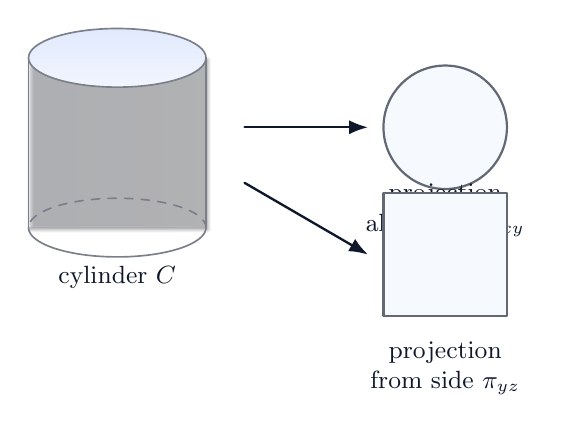
\begin{tikzpicture}[scale=0.98]
  % Cylinder (left) with gentle shading
  \shade[left color=accent!10, right color=accent!3, draw=ink!55, line width=0.6pt, shadow]
    (-1.15,0) rectangle (1.15,-2.2);
  \shade[top color=accent!14, bottom color=accent!6, draw=ink!55, line width=0.6pt]
    (0,0) ellipse (1.15 and 0.38);
  \draw[draw=ink!55, line width=0.6pt] (-1.15,0) -- (-1.15,-2.2);
  \draw[draw=ink!55, line width=0.6pt] (1.15,0) -- (1.15,-2.2);
  \draw[draw=ink!55, line width=0.6pt] (-1.15,-2.2) arc (180:360:1.15 and 0.38);
  \draw[draw=ink!55, line width=0.6pt, dashed] (1.15,-2.2) arc (0:180:1.15 and 0.38);
  \node[annot] at (0,-2.85) {cylinder $C$};

  % Arrows to projections
  \draw[arrow] (1.65,-0.90) -- (3.25,-0.90);
  \draw[arrow] (1.65,-1.62) -- (3.25,-2.55);

  % Circle projection (top-right)
  \draw[draw=ink!65, line width=0.8pt, fill=accent!4] (4.25,-0.90) circle (0.80);
  \node[annot, align=center] at (4.25,-1.98) {projection\\along axis $\pi_{xy}$};

  % Square projection (bottom-right)
  \draw[draw=ink!65, line width=0.8pt, fill=accent!4] (3.45,-3.35) rectangle (5.05,-1.75);
  \node[annot, align=center] at (4.25,-4.02) {projection\\from side $\pi_{yz}$};
\end{tikzpicture}
\caption{A single 3D object can cast different 2D ``shadows'': a cylinder projects to a circle along its axis and to a rectangle/square from the side. This is the geometric intuition behind context-dependent ``views.''}
\label{fig:cylinder-projections}
\end{figure}

\subsection{Why this maps tightly to quantum measurement (Born rule as projection geometry)}

This ``projection resolves apparent contradiction'' story is not merely metaphorical in quantum theory: \textbf{ideal (projective) quantum measurement is literally built from projection operators.}

Let an observable have spectral decomposition
\[
A=\sum_a a\,P_a,
\]
where $P_a$ are orthogonal projectors ($P_aP_{a'}=\delta_{aa'}P_a$, $\sum_a P_a = I$).
For a pure state $|\psi\rangle$, the Born rule can be written as a squared projection norm:
\[
p(a)=\langle\psi|P_a|\psi\rangle=\|P_a|\psi\rangle\|^2.
\]
The post-measurement state (L\"uders rule) is the normalized projection:
\[
|\psi\rangle \;\longrightarrow\; \frac{P_a|\psi\rangle}{\sqrt{p(a)}}.
\]

\begin{figure}[t]
\centering
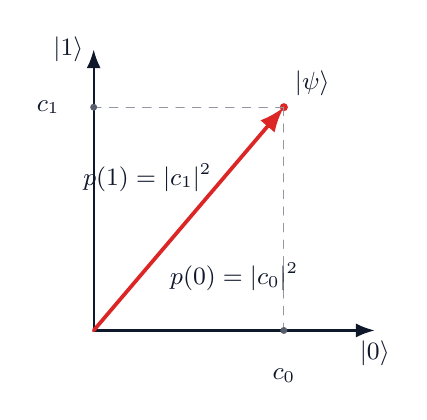
\begin{tikzpicture}[scale=1.05]
  % Basis axes
  \draw[arrow] (0,0) -- (3.4,0) node[below] {$|0\rangle$};
  \draw[arrow] (0,0) -- (0,3.4) node[left] {$|1\rangle$};

  % State vector
  \draw[->, line width=1.35pt, color=accent4] (0,0) -- (2.3,2.7) node[above right] {$|\psi\rangle$};
  \fill[accent4] (2.3,2.7) circle (1.4pt);

  % Projections
  \draw[dashed, color=ink!45] (2.3,2.7) -- (2.3,0);
  \draw[dashed, color=ink!45] (2.3,2.7) -- (0,2.7);
  \fill[ink!70] (2.3,0) circle (1.2pt);
  \fill[ink!70] (0,2.7) circle (1.2pt);

  \node[annot] at (2.3,-0.55) {$c_0$};
  \node[annot] at (-0.55,2.7) {$c_1$};

  \node[annot, align=center] at (1.7,0.65) {$p(0)=|c_0|^2$};
  \node[annot, align=center] at (0.65,1.85) {$p(1)=|c_1|^2$};
\end{tikzpicture}
\caption{Projective measurement as geometric projection. In a chosen basis, a pure state $|\psi\rangle=c_0|0\rangle+c_1|1\rangle$ yields outcome probabilities $|c_0|^2$ and $|c_1|^2$ by the Born rule.}
\label{fig:born-projection}
\end{figure}

So a measurement is, in a precise mathematical sense, a map from a ``higher-dimensional'' object (state vector or density operator) to a lower-dimensional classical outcome, and it generally discards phase/coherence information relative to other incompatible decompositions. Attempting to demand that a system simultaneously carry measurement-independent truth values for multiple incompatible ``views'' is analogous to demanding one 2D shadow be both a circle and a square in the same projection.

\section{Two-level, self-contained guide (fifth grade and graduate level)}

This paper is intentionally written in \emph{two layers}:
\begin{itemize}
  \item \textbf{Layer 1 (fifth grade):} you can read the story and examples without equations.
  \item \textbf{Layer 2 (graduate level):} every key claim is backed by an explicit mathematical model (states, POVMs, Kraus operators) and computed probabilities.
\end{itemize}
Both layers are self-contained: the same ideas appear in simple language first, then in precise form later.

\subsection{Fifth-grade version (no equations required)}

\paragraph{What is Planck time?}
Planck time is a number people get by mixing three ``nature constants'' (how fast light goes, how strong gravity is, and a quantum constant). It is an \emph{extremely} tiny time:
about $0.0000000000000000000000000000000000000000000539$ seconds.

\textbf{Important:} This does \emph{not} mean time is made of tiny ``ticks'' that size. It mainly means: if we try to talk about physics at times that tiny, our usual rules might break because we would need crazy amounts of energy and gravity might matter.

\paragraph{What is a photon?}
In everyday life, light feels like a smooth beam. In modern physics, we often detect light as little ``clicks'' in a sensor. A \textbf{photon} is a name for the smallest unit of light our detectors can register in the right setup.

\textbf{But:} a photon is not like a tiny marble with a clear path you can track without touching it.

\paragraph{What does ``photon on/off'' mean?}
It means we choose a detector and a time window and ask:
\begin{itemize}
  \item \textbf{Off:} no click in that window.
  \item \textbf{On:} a click happens.
\end{itemize}
Even when there is no light, detectors can sometimes click by accident (noise). So ``off'' and ``on'' are really about what the detector does, not a guaranteed label stuck onto the photon.

\paragraph{What is superposition (the big idea)?}
In normal life, a coin is either heads or tails even if you don't look.
In quantum physics, some things are not ``secretly one answer'' before you measure them. Instead, they can be in a special mix called a \textbf{superposition}.

Superposition does \emph{not} mean ``we are confused.'' It means the world can behave in a way where different possibilities can interfere like waves.

\paragraph{A more exact kid definition (and how it differs from guessing).}
\textbf{Definition (kid-level):} A \textbf{superposition} is a special kind of ``both'' where two possibilities are combined in a way that can make \emph{patterns} when they meet again (like waves adding and canceling).

\begin{itemize}
  \item \textbf{Superposition (not just guessing):} The two possibilities can ``work together'' and make interference patterns.
  \item \textbf{Random guessing (a mix):} Sometimes it is one, sometimes the other, but there is no wave-like pattern from them combining.
\end{itemize}

The key idea is: superposition is not only about what you know; it is about what \emph{can be observed} when you set up an experiment that lets the possibilities combine.

\paragraph{How can something look like a square and a circle?}
If you shine a light on a \textbf{cylinder}, its shadow can be a \textbf{circle} from one direction and a \textbf{rectangle} (or even a \textbf{square}) from another direction. The cylinder itself is not a contradiction. The different shadows happen because you are looking from different directions and each shadow throws away information.

Quantum measurements are similar: different measurement setups are like different ``shadows'' of the same underlying quantum state.

\paragraph{Can we look at a photon ``mid-flight''?}
If you do \emph{nothing} in the middle, you only have a math description that tells you the chances of different detector outcomes later.
If you try to look in the middle, you must interact with it (like poking a soap bubble to see where it is). That interaction can change what happens later.

\textbf{So:} ``mid-flight'' does not mean ``it becomes unknowable.'' It means you must say what measurement you use, and that measurement can change the result.

\subsection{Graduate-level map (definitions in one place)}

If you want the precise version immediately, here is the minimal toolkit used throughout:
\begin{itemize}
  \item \textbf{States:} density operators $\rho\ge 0$ with $\Tr(\rho)=1$ on a Hilbert space $\mathcal{H}$.
  \item \textbf{Time evolution:} $\rho(t)=U(t,t_0)\rho(t_0)U^\dagger(t,t_0)$.
  \item \textbf{Measurements:} POVMs $\{E_k\}$ with $E_k\ge 0$ and $\sum_k E_k=I$; outcome probabilities $p(k)=\Tr(\rho E_k)$.
  \item \textbf{Measurement backaction:} instruments/Kraus operators $\{M_k\}$ with $E_k=M_k^\dagger M_k$ and $\rho\mapsto M_k\rho M_k^\dagger/p(k)$.
  \item \textbf{Optical modes:} single-mode ladder operators $a,a^\dagger$ with $[a,a^\dagger]=1$; number operator $N=a^\dagger a$; wavepacket modes $a_f=\int d\omega\,f(\omega)a(\omega)$.
  \item \textbf{On/off detection:} threshold POVM $\Pi_\text{off}=|0\rangle\langle 0|$, $\Pi_\text{on}=I-|0\rangle\langle 0|$, and the standard inefficient model $\Pi_\text{off}^{(\eta)}=\sum_{n\ge 0}(1-\eta)^n|n\rangle\langle n|$.
  \item \textbf{Interference vs.\ which-path:} coherence is carried by off-diagonal terms (e.g.\ $\rho_{AB}$ in the path basis) and is reduced by entanglement or intermediate measurement; quantitatively summarized by visibility--distinguishability tradeoffs (e.g.\ Englert's inequality \cite{englert}).
  \item \textbf{Planck time:} $t_P=\sqrt{\hbar G/c^5}$ (dimensional scale), and heuristic arguments (e.g.\ \cite{salecker_wigner,mead}) suggesting that probing $\Delta t\ll t_P$ pushes required energies toward the Planck scale, where gravitational backreaction cannot be neglected.
\end{itemize}

\subsection{Superposition: explicit definitions (math, physics, and operational)}

This paper uses the word \emph{superposition} in its standard quantum-mechanics sense. Because it is commonly misused in popular discussions, we make the definition explicit in three complementary ways.

\paragraph{Definition 1 (linear combination of state vectors).}
Let $\mathcal{H}$ be a complex Hilbert space. If $|\psi\rangle,|\phi\rangle\in\mathcal{H}$ are state vectors, then any vector
\[
|\chi\rangle = \alpha|\psi\rangle+\beta|\phi\rangle\qquad (\alpha,\beta\in\mathbb{C})
\]
is a \textbf{superposition} (linear combination) of $|\psi\rangle$ and $|\phi\rangle$.
If $|\chi\rangle$ is to represent a physical \emph{pure state}, it is normalized ($\langle\chi|\chi\rangle=1$), and physical states are rays: $|\chi\rangle$ and $e^{\ii\theta}|\chi\rangle$ represent the same pure state (global phase is unobservable).

\paragraph{Definition 2 (superposition in a chosen basis and Born rule meaning).}
Fix an orthonormal basis $\{|i\rangle\}$ of $\mathcal{H}$. Any pure state can be expanded as
\[
|\psi\rangle=\sum_i c_i |i\rangle,\qquad \sum_i |c_i|^2=1.
\]
This is a superposition of basis states with complex amplitudes $c_i$.
If one measures in the $\{|i\rangle\}$ basis (projective measurement with $P_i=|i\rangle\langle i|$), the Born rule gives
\[
p(i)=\langle\psi|P_i|\psi\rangle = |c_i|^2.
\]
The \emph{relative phases} between the $c_i$ (e.g.\ the phase of $c_i c_j^*$) do not affect $p(i)$ in this basis but \emph{do} affect statistics in other measurement contexts (e.g.\ interference measurements), which is the operational content of coherence.

\paragraph{Definition 3 (density-matrix / coherence definition; superposition vs.\ mixture).}
The pure state $|\psi\rangle$ corresponds to $\rho=|\psi\rangle\langle\psi|$. In the basis $\{|i\rangle\}$,
\[
\rho = \sum_{i,j} c_i c_j^*\,|i\rangle\langle j|.
\]
The \textbf{off-diagonal terms} ($i\neq j$) are the \textbf{coherences}. They are the mathematical signature of superposition \emph{relative to that basis}.

By contrast, a classical probabilistic mixture over the same basis states,
\[
\rho_\text{mix}=\sum_i p_i |i\rangle\langle i|,\qquad p_i\ge 0,\ \sum_i p_i=1,
\]
has \emph{no} off-diagonal terms in that basis. Many measurements (including any measurement diagonal in the $\{|i\rangle\}$ basis) cannot distinguish $\rho$ from $\rho_\text{mix}$ if they share the same diagonal elements, but interference-type measurements can.

\begin{figure}[t]
\centering
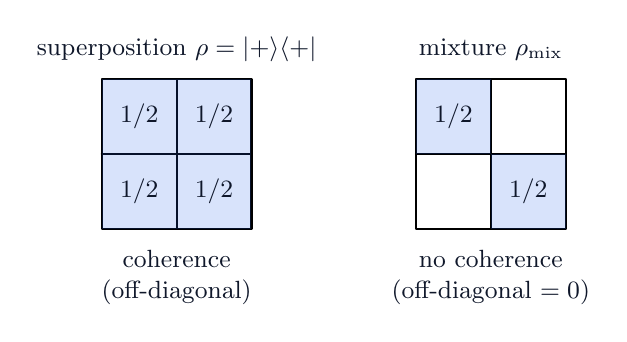
\begin{tikzpicture}[scale=0.95]
  % Left: superposition density matrix (|+><+|)
  \node[annot] at (1.0,2.4) {superposition $\rho=|+\rangle\langle +|$};
  \draw[thick] (0,0) rectangle (2,2);
  \draw[thick] (0,1) -- (2,1);
  \draw[thick] (1,0) -- (1,2);
  \fill[accent, opacity=0.18] (0,0) rectangle (1,1);
  \fill[accent, opacity=0.18] (1,0) rectangle (2,1);
  \fill[accent, opacity=0.18] (0,1) rectangle (1,2);
  \fill[accent, opacity=0.18] (1,1) rectangle (2,2);
  \node[annot] at (0.5,1.5) {$1/2$};
  \node[annot] at (1.5,1.5) {$1/2$};
  \node[annot] at (0.5,0.5) {$1/2$};
  \node[annot] at (1.5,0.5) {$1/2$};
  \node[annot, align=center] at (1.0,-0.65) {coherence\\(off-diagonal)};

  % Right: mixture density matrix (1/2|0><0| + 1/2|1><1|)
  \begin{scope}[xshift=4.2cm]
    \node[annot] at (1.0,2.4) {mixture $\rho_\text{mix}$};
    \draw[thick] (0,0) rectangle (2,2);
    \draw[thick] (0,1) -- (2,1);
    \draw[thick] (1,0) -- (1,2);
    \fill[accent, opacity=0.18] (0,1) rectangle (1,2);
    \fill[accent, opacity=0.18] (1,0) rectangle (2,1);
    \node[annot] at (0.5,1.5) {$1/2$};
    \node[annot] at (1.5,0.5) {$1/2$};
    \node[annot, align=center] at (1.0,-0.65) {no coherence\\(off-diagonal $=0$)};
  \end{scope}
\end{tikzpicture}
\caption{Superposition vs.\ mixture in the density-matrix picture. In a chosen basis, coherent superpositions have off-diagonal terms (coherences) while classical mixtures are diagonal. Interference measurements are sensitive to coherences; purely number-diagonal on/off detection may not be.}
\label{fig:superposition-vs-mixture}
\end{figure}

\paragraph{Operational criterion (how to ``detect'' superposition).}
In practice, one says a system exhibits superposition between alternatives $\{|i\rangle\}$ if there exists a measurement context (often a complementary basis or an interferometric recombination) whose outcome probabilities depend on relative phases and thus on off-diagonal elements of $\rho$ in the $\{|i\rangle\}$ basis. Equivalently: superposition is operationally manifested by \textbf{interference}.

\subsection{Elementary constructions (same idea, two difficulty levels)}

This subsection gives a few \emph{elementary constructions} that work as:
\begin{itemize}
  \item short stories a fifth grader can follow, and
  \item small mathematical models (projections/POVMs) a graduate student can check.
\end{itemize}

\subsubsection{Three polarizers: adding a filter can increase light}

\paragraph{Kid version.}
Imagine you have two pairs of sunglasses. If you rotate one pair sideways compared to the other, almost no light gets through. Now the weird part: if you put a \emph{third} pair of sunglasses in between, tilted halfway, \emph{some} light can get through again. Adding a filter can increase the light!

This is like the cylinder shadow: the middle sunglasses changes the ``question'' being asked of the light.

\begin{figure}[t]
\centering
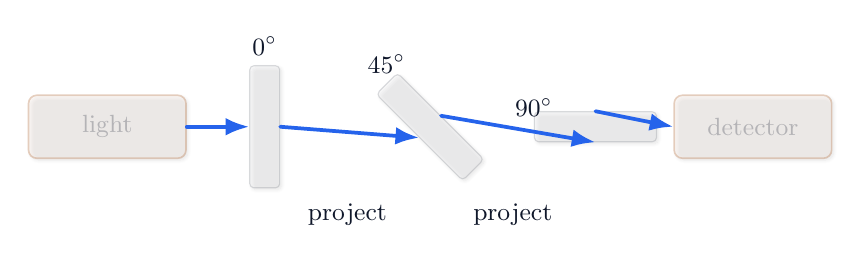
\begin{tikzpicture}[scale=1]
  % Input and output
  \node[blockY] (src) at (0,0) {light};
  \node[blockY] (det) at (8.2,0) {detector};

  % Polarizers
  \node[draw=ink!60, fill=ink!6, rounded corners=1.5pt, minimum width=0.38cm, minimum height=1.55cm, shadow] (P0) at (2.0,0) {};
  \node[draw=ink!60, fill=ink!6, rounded corners=1.5pt, minimum width=0.38cm, minimum height=1.55cm, rotate=45, shadow] (P45) at (4.1,0) {};
  \node[draw=ink!60, fill=ink!6, rounded corners=1.5pt, minimum width=0.38cm, minimum height=1.55cm, rotate=90, shadow] (P90) at (6.2,0) {};

  % Light path
  \draw[light, -{Latex[length=3mm]}] (src.east) -- (P0.west);
  \draw[light, -{Latex[length=3mm]}] (P0.east) -- (P45.west);
  \draw[light, -{Latex[length=3mm]}] (P45.east) -- (P90.west);
  \draw[light, -{Latex[length=3mm]}] (P90.east) -- (det.west);

  % Labels
  \node[annot, above] at (P0.north) {$0^\circ$};
  \node[annot, above] at (P45.north) {$45^\circ$};
  \node[annot, above] at (P90.north) {$90^\circ$};

  \node[annot, below] at (3.05,-0.85) {project};
  \node[annot, below] at (5.15,-0.85) {project};
\end{tikzpicture}
\caption{Three polarizers (``sunglasses'') in sequence. Two crossed polarizers ($0^\circ$ then $90^\circ$) block the beam, but inserting a $45^\circ$ polarizer in between transmits a nonzero fraction (Malus's law).}
\label{fig:three-polarizers}
\end{figure}

\paragraph{Math version (a clean projection example).}
Model polarization as a two-dimensional Hilbert space spanned by horizontal/vertical states $|H\rangle,|V\rangle$. A perfect polarizer at angle $\theta$ transmits the state
\[
|\theta\rangle := \cos\theta\,|H\rangle + \sin\theta\,|V\rangle
\]
and is represented by the projector $P_\theta=|\theta\rangle\langle\theta|$.
If the input is $|H\rangle$, the probability to pass a $\theta$ polarizer is
\[
p=\langle H|P_\theta|H\rangle = |\langle \theta|H\rangle|^2=\cos^2\theta,
\]
which is Malus's law at the single-photon level.

With two crossed polarizers ($0^\circ$ then $90^\circ$), the pass probability is $0$.
With three polarizers ($0^\circ$ then $45^\circ$ then $90^\circ$), the pass probability is
\[
\cos^2(45^\circ)\,\cos^2(45^\circ)=\frac14.
\]
The increase occurs because the intermediate projection changes the state.

\subsubsection{Two paths (interferometer): why ``peeking'' changes the outcome}

\paragraph{Kid version.}
Think of a maze with two paths that split and then join again. If you do not peek, the light can act like a wave and the two routes can ``match up'' so that the photon always exits the same door. If you peek to see which path it took, the peek is a physical interaction and it can ruin the matching, so the exits become more random.

\paragraph{Math version (coherence vs.\ which-path record).}
Represent the two paths by orthonormal states $|A\rangle,|B\rangle$ and consider
\[
|\psi\rangle = \frac{|A\rangle + e^{\ii\phi}|B\rangle}{\sqrt2}.
\]
Interference at recombination depends on the off-diagonal term $\rho_{AB}$ of $\rho=|\psi\rangle\langle\psi|$. If the path becomes correlated with environment states $|E_A\rangle,|E_B\rangle$ with overlap $\gamma=\langle E_B|E_A\rangle$, the interference term is reduced by $|\gamma|$, and output probabilities take the form
\[
P = \frac12\left[1+|\gamma|\cos(\phi-\arg\gamma)\right],
\]
with full visibility at $|\gamma|=1$ and no interference at $|\gamma|=0$.

\subsubsection{On/off vs.\ phase: why a clicker cannot read ``hidden wave-ness''}

\paragraph{Kid version.}
Suppose you only have a simple clicker that tells you ``something arrived'' or ``nothing arrived.'' Two very different situations can look the same to a clicker:
\begin{itemize}
  \item Sometimes there is a little bit of light every time.
  \item Other times, it is \emph{either} no light or a full flash, but mixed randomly.
\end{itemize}
To tell these apart you need a fancier measurement than a click/no-click box.

\paragraph{Math version.}
In the $|0\rangle,|1\rangle$ basis (vacuum vs.\ one-photon), the superposition $|\psi\rangle=(|0\rangle+|1\rangle)/\sqrt2$ and the mixture $\rho_\text{mix}=\tfrac12|0\rangle\langle0|+\tfrac12|1\rangle\langle1|$ have the same number populations but different coherence.
Any on/off POVM diagonal in number (e.g.\ $\Pi_\text{off}^{(\eta)}$) depends only on populations and cannot distinguish them, while quadrature/homodyne statistics (which depend on off-diagonal terms) can.

\subsection{Glossary: kid words \texorpdfstring{$\leftrightarrow$}{<->} physics words}

This table is meant to make the paper self-contained even if you have never seen the formal terms before.

\begin{center}
\begin{tabular}{p{0.28\linewidth} p{0.30\linewidth} p{0.36\linewidth}}
\hline
\textbf{Kid words} & \textbf{Physics words} & \textbf{Meaning (in this paper)} \\
\hline
``Click / no click'' & Threshold detector; POVM & A measurement with two outcomes (on/off). \\
``On/off'' & $\Pi_\text{on},\Pi_\text{off}$; POVM elements & The operators that compute click probabilities. \\
``A photon in flight'' & Evolving state $\rho(t)$ & The mathematical object that predicts future measurement statistics. \\
``Peeking'' & Which-path measurement; environment record & Any interaction that makes path information available and reduces coherence. \\
``Two roads'' & Path basis $\{|A\rangle,|B\rangle\}$ & A two-dimensional subspace describing interferometer arms. \\
``Wave matching'' & Interference; phase coherence & Output depends on off-diagonal terms like $\rho_{AB}$. \\
``Special mix'' & Superposition (pure state) & A coherent combination of possibilities with phase relations. \\
``Random mix'' & Mixed state (density matrix) & Classical uncertainty or entanglement-induced mixture (no coherence). \\
``Different shadows'' & Different measurement bases / projections & Different experimental questions about the same underlying state. \\
``Changing the question changes the answer'' & Context dependence / incompatibility & Different POVMs probe different observables; you cannot demand all answers at once. \\
``Planck time'' & $t_P=\sqrt{\hbar G/c^5}$ & A natural quantum-gravity scale, not automatically a smallest tick. \\
\hline
\end{tabular}
\end{center}

\section{Planck units and Planck time}

\subsection{Dimensional analysis derivation}

We seek a time scale constructed from $\hbar$, $G$, and $c$. Write
\[
t_P \propto \hbar^a G^b c^d.
\]
Using base dimensions:
\[
[\hbar] = \mathrm{M\,L^2\,T^{-1}},\quad
[G] = \mathrm{L^3\,M^{-1}\,T^{-2}},\quad
[c] = \mathrm{L\,T^{-1}}.
\]
We require $\mathrm{T^1}$ overall. Compute:
\begin{itemize}
  \item Mass exponent: $a - b = 0 \Rightarrow a=b$.
  \item Length exponent: $2a + 3b + d = 0 \Rightarrow 2a + 3a + d = 0 \Rightarrow d=-5a$.
  \item Time exponent: $-a - 2b - d = 1 \Rightarrow -a - 2a - (-5a) = 1 \Rightarrow 2a = 1 \Rightarrow a=b=\tfrac12$.
\end{itemize}
Thus $d=-\tfrac{5}{2}$ and
\[
t_P = \sqrt{\frac{\hbar G}{c^5}}.
\]

\subsection{Numerical value and associated scales}

Using (approximately):
\[
\hbar \approx 1.054571817\times 10^{-34}\,\mathrm{J\,s},\quad
G \approx 6.67430\times 10^{-11}\,\mathrm{m^3\,kg^{-1}\,s^{-2}},\quad
c = 2.99792458\times 10^8\,\mathrm{m\,s^{-1}},
\]
we obtain:
\[
t_P \approx 5.39\times 10^{-44}\,\mathrm{s}.
\]
Related Planck units:
\[
\ell_P=\sqrt{\frac{\hbar G}{c^3}}\approx 1.62\times 10^{-35}\,\mathrm{m},\quad
m_P=\sqrt{\frac{\hbar c}{G}}\approx 2.18\times 10^{-8}\,\mathrm{kg},
\]
\[
E_P=m_Pc^2=\sqrt{\frac{\hbar c^5}{G}}\approx 1.96\times 10^9\,\mathrm{J}\approx 1.22\times 10^{19}\,\mathrm{GeV}.
\]
Note the identity $E_P = \hbar/t_P$.

\subsection{What Planck time does (and does not) imply}
\paragraph{Plain-language interpretation.}
Planck units are not ``measured constants'' like the speed of light; they are \emph{constructed} by combining constants we already know. Their value tells you roughly where different parts of physics may collide. Here is the safe operational message:
\begin{itemize}
  \item When you push time-resolution requirements smaller, you typically need larger bandwidth and larger energies.
  \item If the required energies become large enough, gravity cannot be treated as a small background effect.
\end{itemize}
Planck time is the natural scale where this crossover is expected to become unavoidable.

\begin{itemize}
  \item \textbf{Does imply:} a natural scale where the dimensionless combination of couplings suggests quantum-gravity effects may be important.
  \item \textbf{Does not (by itself) imply:} that time is fundamentally discrete in steps of $t_P$, or that physical systems must ``update'' at that cadence, or that any particular ``on/off'' predicate must flip on Planck timescales.
\end{itemize}

\subsection{Heuristic ``minimum time'' from quantum localization + gravity (careful)}

A standard heuristic combines:
\begin{enumerate}
  \item To operationally probe time resolution $\Delta t$, one needs frequency components with $\Delta\omega \gtrsim 1/\Delta t$ (Fourier limitation).
  \item Quanta at angular frequency $\omega$ have energy $\sim \hbar\omega$, so resolving $\Delta t$ pushes energies toward $E \sim \hbar/\Delta t$ (order-of-magnitude).
  \item Concentrating energy $E$ within a region of size $R\sim c\Delta t$ yields an associated Schwarzschild radius
  \[
  r_s = \frac{2GE}{c^4}.
  \]
\end{enumerate}

Requiring $r_s \lesssim R$ (avoid immediate horizon formation in this crude model) gives:
\[
\frac{2GE}{c^4} \lesssim c\Delta t.
\]
Insert $E\sim \hbar/\Delta t$:
\[
\frac{2G\hbar}{c^4\,\Delta t} \lesssim c\Delta t
\;\Rightarrow\;
\Delta t^2 \gtrsim \frac{2\hbar G}{c^5}
\;\Rightarrow\;
\Delta t \gtrsim \sqrt{2}\,t_P.
\]
\textbf{Interpretation:} this is a plausibility argument that sub-Planckian operational time resolution may require energies at which gravitational backreaction becomes non-negligible. It is not a derivation of time discreteness or a theorem of quantum theory alone.

\section{Quantized optical modes: ``what is a photon?''}

In quantum optics, a ``photon'' is most cleanly defined as an excitation of a \textbf{mode} of the electromagnetic field. A ``mode'' is not unique: it depends on boundary conditions (cavity/waveguide), filtering, pulse shaping, detection mode-matching, etc.

\subsection{Modes in everyday terms (why ``a photon'' needs a context)}
In everyday language, ``light'' sounds like one thing. In experiments, it is more like \emph{many possible channels}:
\begin{itemize}
  \item A radio has many stations; saying ``there is music'' is incomplete unless you say \emph{which station} you tuned to.
  \item A guitar string can vibrate in different harmonics; saying ``the string is vibrating'' is incomplete unless you say \emph{which pattern} of vibration.
\end{itemize}
In quantum optics, a \textbf{mode} plays the role of the ``station'' or the ``vibration pattern.'' A detector, together with filters and geometry, effectively chooses which mode it is sensitive to. This is why the question ``is there a photon?'' must be read as ``is there a photon in \emph{this} mode that my apparatus couples to?''

\begin{figure}[t]
\centering
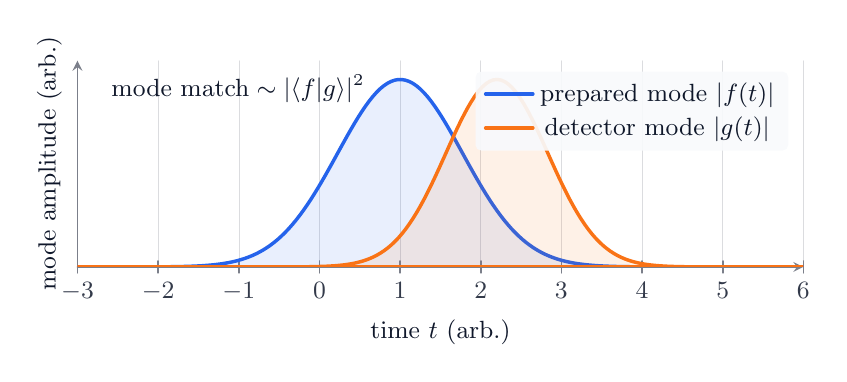
\begin{tikzpicture}
\begin{axis}[
  width=10.8cm,
  height=4.2cm,
  xlabel={time $t$ (arb.)},
  ylabel={mode amplitude (arb.)},
  xmin=-3, xmax=6,
  ymin=0, ymax=1.1,
  axis lines=left,
  legend style={at={(0.98,0.95)}, anchor=north east},
  ytick=\empty
]
\addplot[draw=accent, fill=accent, fill opacity=0.10, domain=-3:6, samples=200] {exp(-(x-1)^2/1.2)} \closedcycle;
\addlegendentry{prepared mode $|f(t)|$}
\addplot[draw=accent2, fill=accent2, fill opacity=0.10, domain=-3:6, samples=200] {exp(-(x-2.2)^2/0.8)} \closedcycle;
\addlegendentry{detector mode $|g(t)|$}
\node[anchor=west] at (axis cs:-2.7,0.95) {$\text{mode match} \sim |\langle f|g\rangle|^2$};
\end{axis}
\end{tikzpicture}
\caption{Mode matching intuition. A source prepares a pulse shape (blue) while a detector is sensitive to a (possibly different) mode (red). Click probabilities depend on their overlap, often behaving like an additional efficiency factor.}
\label{fig:mode-matching}
\end{figure}

\subsection{Single-mode field algebra}
For a single bosonic mode:
\[
[a,a^\dagger]=1,\quad N=a^\dagger a.
\]
The Fock basis $\{|n\rangle\}_{n=0}^\infty$ satisfies:
\[
N|n\rangle=n|n\rangle,\quad
a|n\rangle=\sqrt{n}\,|n-1\rangle,\quad
a^\dagger|n\rangle=\sqrt{n+1}\,|n+1\rangle.
\]

\subsection{Canonical states}
\begin{itemize}
  \item \textbf{Vacuum:} $|0\rangle$.
  \item \textbf{Number (Fock) state:} $|n\rangle$ with definite photon number $n$.
  \item \textbf{Coherent state:} $|\alpha\rangle$ defined by $a|\alpha\rangle=\alpha|\alpha\rangle$. Expansion:
  \[
  |\alpha\rangle = e^{-|\alpha|^2/2}\sum_{n=0}^\infty \frac{\alpha^n}{\sqrt{n!}}|n\rangle.
  \]
  Photon number distribution:
  \[
  P(n)=|\langle n|\alpha\rangle|^2=e^{-|\alpha|^2}\frac{|\alpha|^{2n}}{n!},
  \]
  i.e.\ Poisson with mean $\mu=|\alpha|^2$.
  \item \textbf{Thermal state:} diagonal in number basis with Bose--Einstein distribution. If mean photon number is $\bar n$:
  \[
  \rho_\text{th}=\sum_{n=0}^\infty \frac{\bar n^n}{(1+\bar n)^{n+1}}|n\rangle\langle n|.
  \]
\end{itemize}

\subsection{Wavepacket modes (time/frequency localized photons)}
For a continuum of frequency modes with operators $a(\omega)$ satisfying
\[
[a(\omega),a^\dagger(\omega')]=\delta(\omega-\omega'),
\]
define a normalized wavepacket mode $f(\omega)$ with $\int d\omega\,|f(\omega)|^2=1$ and
\[
a_f = \int d\omega\, f(\omega)\,a(\omega),\quad [a_f,a_f^\dagger]=1.
\]
Then $|1_f\rangle = a_f^\dagger|0\rangle$ is ``one photon in mode $f$.'' Crucially, different choices of $f$ define different ``photon number'' questions.

\section{What does ``on/off'' mean? Explicit measurement models}

\subsection{Plain-language version: what a click/no-click detector really tells you}
Many real photon detectors are \emph{threshold devices}: they do not output ``there were exactly $n$ photons.'' They output something closer to:
\begin{itemize}
  \item ``I registered an event in this time window'' (click), or
  \item ``I did not register an event'' (no click).
\end{itemize}
Two practical facts follow:
\begin{itemize}
  \item \textbf{No click does not prove vacuum.} You might have missed the photon (loss/inefficiency), or it arrived outside the window, or it did not match the detector mode.
  \item \textbf{A click does not prove exactly one photon.} Threshold detectors often cannot distinguish one photon from two.
\end{itemize}
The POVM formalism below is simply the clean mathematical way to encode these operational realities.

\begin{figure}[t]
\centering
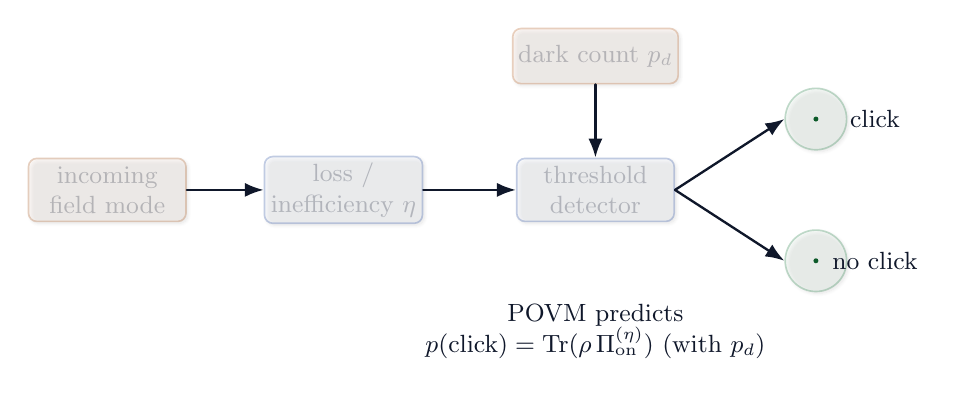
\begin{tikzpicture}[scale=1.0]
  \node[blockY] (in) at (0,0) {incoming\\field mode};
  \node[block] (loss) at (3.0,0) {loss /\\inefficiency $\eta$};
  \node[block] (det) at (6.2,0) {threshold\\detector};

  \node[detector] (click) at (9.0,0.9) {};
  \node[detector] (noclick) at (9.0,-0.9) {};
  \fill[accent3!55!black] (click.center) circle (0.9pt);
  \fill[accent3!55!black] (noclick.center) circle (0.9pt);
  \node[annot] at (9.75,0.9) {click};
  \node[annot] at (9.75,-0.9) {no click};

  \draw[arrow] (in.east) -- (loss.west);
  \draw[arrow] (loss.east) -- (det.west);
  \draw[arrow] (det.east) -- (click.west);
  \draw[arrow] (det.east) -- (noclick.west);

  % Dark count
  \node[phase] (dark) at (6.2,1.7) {dark count $p_d$};
  \draw[arrow] (dark.south) -- (det.north);

  \node[annot, align=center] at (6.2,-1.8) {POVM predicts\\$p(\text{click})=\Tr(\rho\,\Pi_\text{on}^{(\eta)})$ (with $p_d$)};
\end{tikzpicture}
\caption{Operational picture of ``on/off'' detection. A click/no-click outcome depends on detector efficiency (loss/mode mismatch) and noise (dark counts). The POVM formalism encodes this as outcome probabilities derived from the state $\rho$.}
\label{fig:onoff-detector}
\end{figure}

\subsection{Photon number projective measurement vs.\ on/off detection}
An ideal number-resolving measurement uses projectors $\Pi_n = |n\rangle\langle n|$.
An \textbf{ideal on/off detector} (threshold detector) distinguishes only:
\begin{itemize}
  \item ``off'' $=$ vacuum ($n=0$),
  \item ``on'' $=$ any nonzero photon number ($n\ge 1$).
\end{itemize}
The corresponding POVM elements are:
\[
\Pi_\text{off} = |0\rangle\langle 0|,\quad
\Pi_\text{on} = I - |0\rangle\langle 0|.
\]
For a state $\rho$, predicted probabilities:
\[
p_\text{off}=\Tr(\rho\,\Pi_\text{off}),\quad
p_\text{on}=\Tr(\rho\,\Pi_\text{on})=1-p_\text{off}.
\]

\subsection{Inefficiency and dark counts (standard quantum-optics model)}
Let $\eta\in[0,1]$ be detection efficiency. A common model treats each photon as independently detected with probability $\eta$. Then the probability of \textbf{no click} given $n$ photons is $(1-\eta)^n$.
This corresponds to the POVM:
\[
\Pi_\text{off}^{(\eta)}=\sum_{n=0}^\infty (1-\eta)^n\,|n\rangle\langle n|,
\quad
\Pi_\text{on}^{(\eta)}=I-\Pi_\text{off}^{(\eta)}.
\]
Add a dark-count probability $p_d$ per detection window by mixing with a classical ``false click'':
\[
p_\text{off} = (1-p_d)\,\Tr(\rho\,\Pi_\text{off}^{(\eta)}),
\quad
p_\text{on}=1-p_\text{off}.
\]

\subsection{Immediate consequence: phases can be invisible to on/off}
Because $\Pi_\text{off}^{(\eta)}$ is diagonal in the number basis, any relative phase between $|0\rangle$ and $|1\rangle$ in a superposition $\alpha|0\rangle+\beta|1\rangle$ will not affect $p_\text{on/off}$. To see that phase, one needs a different measurement (e.g.\ homodyne).

\section{Scenarios with explicit calculations}

\subsection{A few plug-in numbers (intuition without new concepts)}
This subsection gives ``back of the envelope'' numbers using formulas derived later, so a general reader can build intuition quickly.

\paragraph{Example 1: weak coherent pulse and click probability.}
For a coherent state with mean photon number $\mu$ and detector efficiency $\eta$ (no dark counts), we derive
\[
p_\text{on}=1-e^{-\eta\mu}.
\]
If $\mu=0.2$ (a very dim pulse) and $\eta=0.6$, then $\eta\mu=0.12$ and
\[
p_\text{on}=1-e^{-0.12}\approx 0.113.
\]
So even though ``on average'' there are $0.2$ photons in the mode, most windows produce no click, and about $11\%$ click.

\paragraph{Example 2: vacuum with dark counts.}
If the true state is vacuum but the detector has a dark-count probability $p_d=0.01$ per window, then $p_\text{on}=p_d=1\%$. This is one reason you must not treat clicks as infallible metaphysical events; they are outcomes of a noisy physical device.

\subsection{Vacuum vs.\ one-photon Fock state}
Let $\rho=|0\rangle\langle0|$. With ideal on/off:
\[
p_\text{off}=1,\quad p_\text{on}=0.
\]
With inefficiency and dark counts:
\[
\Tr(\rho\,\Pi_\text{off}^{(\eta)}) = (1-\eta)^0 = 1
\Rightarrow
p_\text{on} = 1-(1-p_d)\cdot 1 = p_d.
\]
So even vacuum can ``click'' due to dark counts.

Now take $\rho=|1\rangle\langle1|$. Then
\[
\Tr(\rho\,\Pi_\text{off}^{(\eta)})=(1-\eta)^1 = 1-\eta
\Rightarrow
p_\text{on}=1-(1-p_d)(1-\eta)=p_d + (1-p_d)\eta.
\]
For $p_d=0$, $p_\text{on}=\eta$: a one-photon state does not guarantee a click unless $\eta=1$.

\subsection{The clearest ``on/off superposition'': \texorpdfstring{$|\psi\rangle=\alpha|0\rangle+\beta|1\rangle$}{|psi> = alpha|0> + beta|1>}}
Let $|\alpha|^2+|\beta|^2=1$ and $\rho=|\psi\rangle\langle\psi|$.
Because $\Pi_\text{off}^{(\eta)}$ is diagonal in $|n\rangle$,
\[
\Tr(\rho\,\Pi_\text{off}^{(\eta)})
= |\alpha|^2(1-\eta)^0 + |\beta|^2(1-\eta)^1
= |\alpha|^2 + (1-\eta)|\beta|^2
= 1-\eta|\beta|^2.
\]
Thus (with $p_d=0$):
\[
p_\text{on}=\eta|\beta|^2.
\]
With ideal detection $\eta=1$, $p_\text{on}=|\beta|^2$.

\subsubsection{On/off cannot see coherence; homodyne (quadrature) can (explicit calculation)}
The on/off POVM depends only on the populations $\rho_{nn}$. This means a coherent superposition and an incoherent mixture can have identical on/off statistics. Define the mixture
\[
\rho_\text{mix} := |\alpha|^2|0\rangle\langle 0| + |\beta|^2|1\rangle\langle 1|.
\]
Then for either $\rho=|\psi\rangle\langle\psi|$ or $\rho_\text{mix}$,
\[
p_\text{on} = 1-\Tr(\rho\,\Pi_\text{off}^{(\eta)}) = \eta|\beta|^2.
\]

To see the difference, consider a homodyne (quadrature) measurement. Define the dimensionless quadrature operator
\[
X := \frac{a+a^\dagger}{\sqrt{2}},
\]
with eigenstates $|x\rangle$ satisfying $X|x\rangle=x|x\rangle$.
In the $x$-representation, the first two harmonic-oscillator wavefunctions are:
\[
\psi_0(x):=\langle x|0\rangle = \pi^{-1/4}e^{-x^2/2},\qquad
\psi_1(x):=\langle x|1\rangle = \pi^{-1/4}\sqrt{2}\,x\,e^{-x^2/2}.
\]
For the pure state $|\psi\rangle=\alpha|0\rangle+\beta|1\rangle$,
\[
\langle x|\psi\rangle=\alpha\psi_0(x)+\beta\psi_1(x)
=\pi^{-1/4}e^{-x^2/2}\left(\alpha+\sqrt{2}\,x\,\beta\right),
\]
so the probability density is
\[
P_\psi(x)=|\langle x|\psi\rangle|^2
=\pi^{-1/2}e^{-x^2}\left(|\alpha|^2 + 2x^2|\beta|^2 + 2\sqrt{2}\,x\,\mathrm{Re}(\alpha^*\beta)\right).
\]
For the mixture,
\[
P_\text{mix}(x)=\Tr(\rho_\text{mix}|x\rangle\langle x|)
=\pi^{-1/2}e^{-x^2}\left(|\alpha|^2 + 2x^2|\beta|^2\right),
\]
which lacks the linear ``interference'' term proportional to $\mathrm{Re}(\alpha^*\beta)$. Thus coherence (and relative phase) is operationally accessible in quadrature statistics even though it is invisible to on/off detection. In practice one measures a phase-rotated quadrature $X_\varphi=(a e^{-\ii\varphi}+a^\dagger e^{\ii\varphi})/\sqrt2$ by varying the local-oscillator phase $\varphi$.

\subsection{Coherent state \texorpdfstring{$|\alpha\rangle$}{|alpha>}: Poisson counting \texorpdfstring{$\Rightarrow$}{=>} closed-form click probability}
For $\rho=|\alpha\rangle\langle\alpha|$ with mean photon number $\mu=|\alpha|^2$,
\[
\Tr(\rho\,\Pi_\text{off}^{(\eta)})
=\sum_{n=0}^\infty (1-\eta)^n\,P(n)
=\sum_{n=0}^\infty (1-\eta)^n\,e^{-\mu}\frac{\mu^n}{n!}.
\]
Recognize the exponential series:
\[
\Tr(\rho\,\Pi_\text{off}^{(\eta)})
= e^{-\mu}\sum_{n=0}^\infty \frac{\left((1-\eta)\mu\right)^n}{n!}
= e^{-\mu}\,e^{(1-\eta)\mu}
= e^{-\eta\mu}.
\]
So (with dark counts $p_d$):
\[
p_\text{on}=1-(1-p_d)e^{-\eta\mu}.
\]

\begin{figure}[t]
\centering
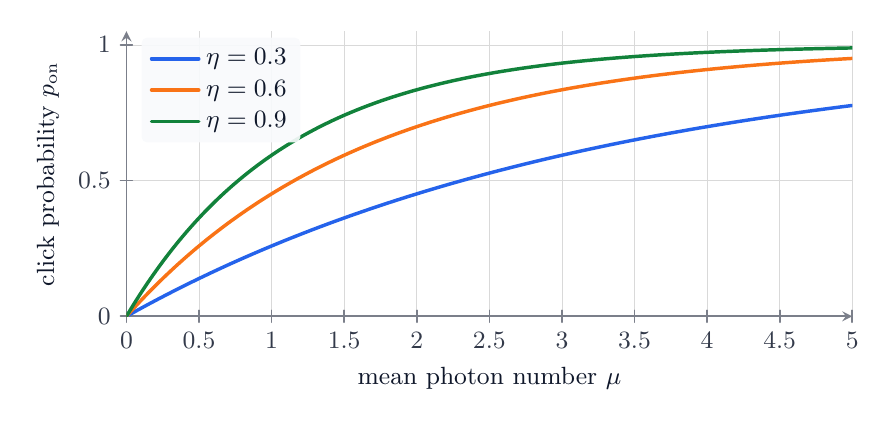
\begin{tikzpicture}
\begin{axis}[
  width=10.8cm,
  height=5.2cm,
  xlabel={mean photon number $\mu$},
  ylabel={click probability $p_\text{on}$},
  xmin=0, xmax=5,
  ymin=0, ymax=1.05,
  axis lines=left,
  legend style={at={(0.02,0.98)}, anchor=north west, font=\small},
  grid=both,
  grid style={line width=.1pt, draw=gray!20},
  major grid style={line width=.2pt,draw=gray!30}
]
\addplot[accent, domain=0:5, samples=200] {1-exp(-0.3*x)};
\addlegendentry{$\eta=0.3$}
\addplot[accent2, domain=0:5, samples=200] {1-exp(-0.6*x)};
\addlegendentry{$\eta=0.6$}
\addplot[accent3!80!black, domain=0:5, samples=200] {1-exp(-0.9*x)};
\addlegendentry{$\eta=0.9$}
\end{axis}
\end{tikzpicture}
\caption{Click probability for a coherent state with mean photon number $\mu$ and detector efficiency $\eta$ (here with $p_d=0$): $p_\text{on}=1-e^{-\eta\mu}$. Even ``brightening'' the pulse slightly can change click rates substantially when $\mu$ is small.}
\label{fig:click-probability}
\end{figure}

\subsection{Thermal state \texorpdfstring{$\rho_\text{th}$}{rho-th}: click probability and heavy tails}
For $\rho=\rho_\text{th}$ with mean $\bar n$,
\[
\Tr(\rho\,\Pi_\text{off}^{(\eta)})
=\sum_{n=0}^\infty (1-\eta)^n\,\frac{\bar n^n}{(1+\bar n)^{n+1}}
=\frac{1}{1+\bar n}\sum_{n=0}^\infty \left(\frac{(1-\eta)\bar n}{1+\bar n}\right)^n.
\]
This is a geometric series with ratio $r=\frac{(1-\eta)\bar n}{1+\bar n}$, so
\[
\Tr(\rho\,\Pi_\text{off}^{(\eta)})
=\frac{1}{1+\eta\bar n}.
\]
Thus (with $p_d=0$):
\[
p_\text{on}=1-\frac{1}{1+\eta\bar n}=\frac{\eta\bar n}{1+\eta\bar n}.
\]

\begin{figure}[t]
\centering
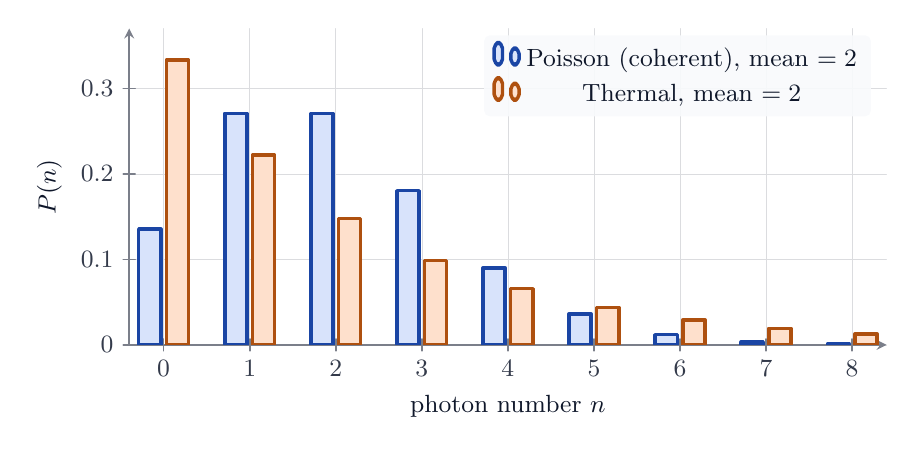
\begin{tikzpicture}
\begin{axis}[
  width=11.2cm,
  height=5.6cm,
  ybar,
  bar width=8pt,
  xlabel={photon number $n$},
  ylabel={$P(n)$},
  symbolic x coords={0,1,2,3,4,5,6,7,8},
  xtick=data,
  ymin=0, ymax=0.37,
  axis lines=left,
  legend style={at={(0.98,0.98)}, anchor=north east},
  enlarge x limits=0.05
]
\addplot[fill=accent!18, draw=accent!70!black] coordinates {
  (0,0.1353) (1,0.2707) (2,0.2707) (3,0.1804) (4,0.0902) (5,0.0361) (6,0.0120) (7,0.0034) (8,0.0009)
};
\addlegendentry{Poisson (coherent), mean $=2$}
\addplot[fill=accent2!22, draw=accent2!70!black] coordinates {
  (0,0.3333) (1,0.2222) (2,0.1481) (3,0.0988) (4,0.0658) (5,0.0439) (6,0.0293) (7,0.0195) (8,0.0130)
};
\addlegendentry{Thermal, mean $=2$}
\end{axis}
\end{tikzpicture}
\caption{Photon-number distributions for two common light states with the same mean photon number. A coherent state has a Poisson distribution (narrower tail), while a thermal state is broader (heavier tail). ``On/off'' detectors collapse this detail into a single click/no-click outcome.}
\label{fig:number-distributions}
\end{figure}

\subsection{Mach--Zehnder interferometer: single-photon interference vs.\ which-path information}
We model two spatial modes (arms) $A$ and $B$ with creation operators $a^\dagger, b^\dagger$.

\begin{figure}[t]
\centering
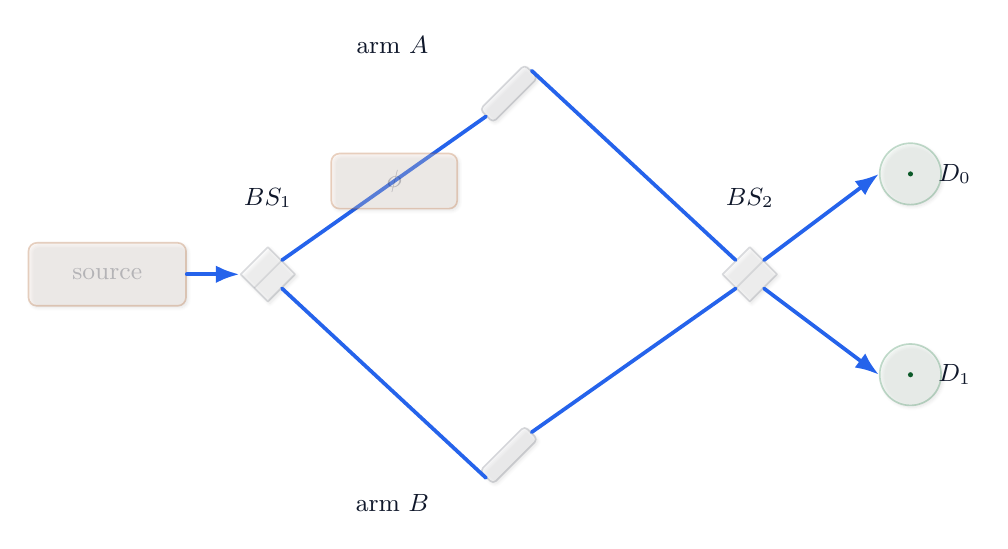
\begin{tikzpicture}[scale=1.02]
  % Nodes
  \node[blockY] (src) at (-2,0) {source};
  \node[bs] (bs1) at (0,0) {};
  \node[bs] (bs2) at (6,0) {};
  \node[detector] (d0) at (8,1.25) {};
  \node[detector] (d1) at (8,-1.25) {};
  \fill[accent3!55!black] (d0.center) circle (0.9pt);
  \fill[accent3!55!black] (d1.center) circle (0.9pt);
  \node[annot] at (8.55,1.25) {$D_0$};
  \node[annot] at (8.55,-1.25) {$D_1$};

  % Mirrors
  \node[mirror] (m1) at (3,2.25) {};
  \node[mirror] (m2) at (3,-2.25) {};

  % Paths (use node anchors for clean geometry)
  \draw[light, -{Latex[length=3mm]}] (src.east) -- (bs1.west);

  \draw[light] (bs1.north east) -- node[phase, pos=0.55] {$\phi$} (m1.west);
  \draw[light] (m1.east) -- (bs2.north west);

  \draw[light] (bs1.south east) -- (m2.west);
  \draw[light] (m2.east) -- (bs2.south west);

  \draw[light, -{Latex[length=3mm]}] (bs2.north east) -- (d0.west);
  \draw[light, -{Latex[length=3mm]}] (bs2.south east) -- (d1.west);

  % Labels
  \node[annot] at (1.55,2.85) {arm $A$};
  \node[annot] at (1.55,-2.85) {arm $B$};
  \node[annot] at (0,0.95) {$BS_1$};
  \node[annot] at (6,0.95) {$BS_2$};
\end{tikzpicture}
\caption{Mach--Zehnder interferometer schematic. A single photon entering $BS_1$ is put into a superposition of two paths (arms $A$ and $B$). A relative phase $\phi$ affects output click probabilities at detectors $D_0,D_1$ when coherence is preserved.}
\label{fig:mzi}
\end{figure}

\subsubsection{50/50 beamsplitter transformation (one convention)}
Let the first beamsplitter implement:
\[
U_\text{BS}^\dagger a\,U_\text{BS}=\frac{a+\ii b}{\sqrt{2}},\quad
U_\text{BS}^\dagger b\,U_\text{BS}=\frac{\ii a+b}{\sqrt{2}}.
\]
Input state: one photon in mode $a$, vacuum in $b$:
\[
|\psi_\text{in}\rangle = |1\rangle_a|0\rangle_b = a^\dagger|0\rangle.
\]
After the first beamsplitter:
\[
|\psi_1\rangle = U_\text{BS}|\psi_\text{in}\rangle
= \left(\frac{a^\dagger - \ii b^\dagger}{\sqrt{2}}\right)|0\rangle
= \frac{|1,0\rangle - \ii|0,1\rangle}{\sqrt{2}}.
\]
Apply a phase shift $\phi$ in arm $B$: $b^\dagger\mapsto e^{\ii\phi} b^\dagger$:
\[
|\psi_\phi\rangle=\frac{|1,0\rangle - \ii e^{\ii\phi}|0,1\rangle}{\sqrt{2}}.
\]
After the second identical beamsplitter, define output modes:
\[
c=\frac{a+\ii b}{\sqrt{2}},\quad d=\frac{\ii a+b}{\sqrt{2}}
\Rightarrow
a=\frac{c-\ii d}{\sqrt{2}},\quad b=\frac{-\ii c+d}{\sqrt{2}}.
\]
Using
\[
a^\dagger=\frac{c^\dagger+\ii d^\dagger}{\sqrt{2}},\quad
b^\dagger=\frac{\ii c^\dagger+d^\dagger}{\sqrt{2}},
\]
we have
\[
|\psi_\phi\rangle
=\frac{1}{\sqrt{2}}\left(a^\dagger - \ii e^{\ii\phi} b^\dagger\right)|0\rangle
=\frac{1}{\sqrt{2}}\left(
\frac{c^\dagger+\ii d^\dagger}{\sqrt{2}}
- \ii e^{\ii\phi}\frac{\ii c^\dagger+d^\dagger}{\sqrt{2}}
\right)|0\rangle.
\]
Simplify the bracket:
\[
\frac{1}{\sqrt{2}}\left(
\frac{c^\dagger+\ii d^\dagger}{\sqrt{2}}
+\frac{e^{\ii\phi} c^\dagger - \ii e^{\ii\phi} d^\dagger}{\sqrt{2}}
\right)
=\frac{1}{2}\left(
(1+e^{\ii\phi})c^\dagger + \ii(1-e^{\ii\phi})d^\dagger
\right).
\]
Thus:
\[
|\psi_\text{out}\rangle
=\frac{1+e^{\ii\phi}}{2}|1\rangle_c|0\rangle_d
+\frac{\ii(1-e^{\ii\phi})}{2}|0\rangle_c|1\rangle_d.
\]
Therefore detection probabilities:
\[
P(c)=\left|\frac{1+e^{\ii\phi}}{2}\right|^2
=\frac{1+\cos\phi}{2}=\cos^2\left(\frac{\phi}{2}\right),
\]
\[
P(d)=\left|\frac{1-e^{\ii\phi}}{2}\right|^2
=\frac{1-\cos\phi}{2}=\sin^2\left(\frac{\phi}{2}\right).
\]

\subsubsection{Which-path information as dephasing: interference disappears}
Suppose the path becomes entangled with an environment/pointer state $|E_A\rangle,|E_B\rangle$:
\[
|\Psi\rangle = \frac{|1,0\rangle|E_A\rangle - \ii|0,1\rangle|E_B\rangle}{\sqrt{2}}.
\]
If $\langle E_A|E_B\rangle=0$, tracing out the environment yields:
\[
\rho_{AB}=\Tr_E(|\Psi\rangle\langle\Psi|)
=\frac12\left(|1,0\rangle\langle 1,0| + |0,1\rangle\langle 0,1|\right),
\]
with no coherence. Propagating this mixture through the phase shifter and second beamsplitter yields $P(c)=P(d)=\tfrac12$, independent of $\phi$.

\begin{figure}[t]
\centering
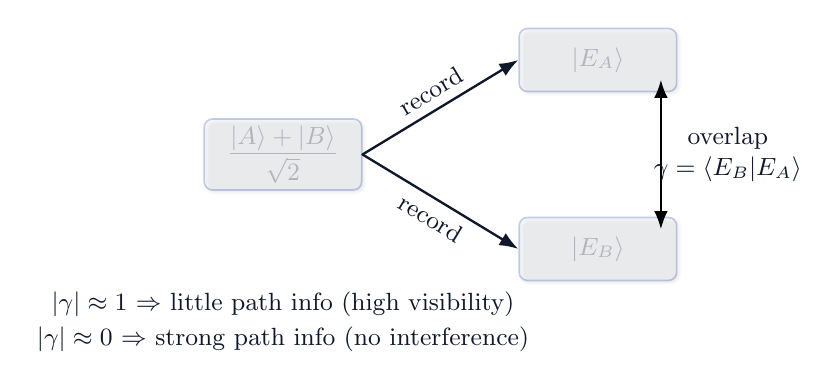
\begin{tikzpicture}[scale=1.0]
  \node[block] (split) at (0,0) {$\displaystyle \frac{|A\rangle+|B\rangle}{\sqrt2}$};
  \node[block] (EA) at (4,1.2) {$|E_A\rangle$};
  \node[block] (EB) at (4,-1.2) {$|E_B\rangle$};

  \draw[arrow] (split.east) -- node[annot, above, sloped] {record} (EA.west);
  \draw[arrow] (split.east) -- node[annot, below, sloped] {record} (EB.west);

  \draw[<->, thick] (4.8,0.95) -- (4.8,-0.95);
  \node[annot, align=center] at (5.65,0) {overlap\\$\gamma=\langle E_B|E_A\rangle$};

  \node[annot] at (0,-1.9) {$|\gamma|\approx 1$ $\Rightarrow$ little path info (high visibility)};
  \node[annot] at (0,-2.35) {$|\gamma|\approx 0$ $\Rightarrow$ strong path info (no interference)};
\end{tikzpicture}
\caption{Partial which-path information: visibility depends on the overlap $\gamma=\langle E_B|E_A\rangle$ of the environment records correlated with each path.}
\label{fig:which-path-overlap}
\end{figure}

\subsubsection{Partial which-path information: overlap controls visibility and yields a quantitative tradeoff}
Let $\gamma := \langle E_B|E_A\rangle$, with $0\le |\gamma|\le 1$, and include a phase shift $\phi$ in arm $B$:
\[
|\Psi_\phi\rangle=\frac{|1,0\rangle|E_A\rangle - \ii e^{\ii\phi}|0,1\rangle|E_B\rangle}{\sqrt{2}}.
\]
Tracing out the environment yields
\[
\rho_{AB}
=\frac12\Big(
|1,0\rangle\langle 1,0| + |0,1\rangle\langle 0,1|
+ \ii\gamma e^{-\ii\phi}|1,0\rangle\langle 0,1|
- \ii\gamma^* e^{\ii\phi}|0,1\rangle\langle 1,0|
\Big).
\]
Using $c=(a+\ii b)/\sqrt2$ so that
\[
n_c=c^\dagger c=\frac{a^\dagger a + b^\dagger b + \ii a^\dagger b - \ii b^\dagger a}{2},
\]
one obtains
\[
P(c)=\frac12\left[1+|\gamma|\cos\!\left(\phi-\arg\gamma\right)\right],
\]
so the fringe visibility is $V=|\gamma|$.

The best possible which-path guess from the environment record is a binary state discrimination problem between $|E_A\rangle$ and $|E_B\rangle$ with equal priors. Helstrom's bound gives \cite{helstrom}
\[
P_\text{succ}^\star=\frac12\left(1+\sqrt{1-|\langle E_A|E_B\rangle|^2}\right)
=\frac12\left(1+\sqrt{1-|\gamma|^2}\right).
\]
Define distinguishability $D:=2P_\text{succ}^\star-1=\sqrt{1-|\gamma|^2}$. Therefore
\[
V^2 + D^2 = 1
\]
in this pure-state model (more general models give $V^2 + D^2 \le 1$).

\begin{figure}[t]
\centering
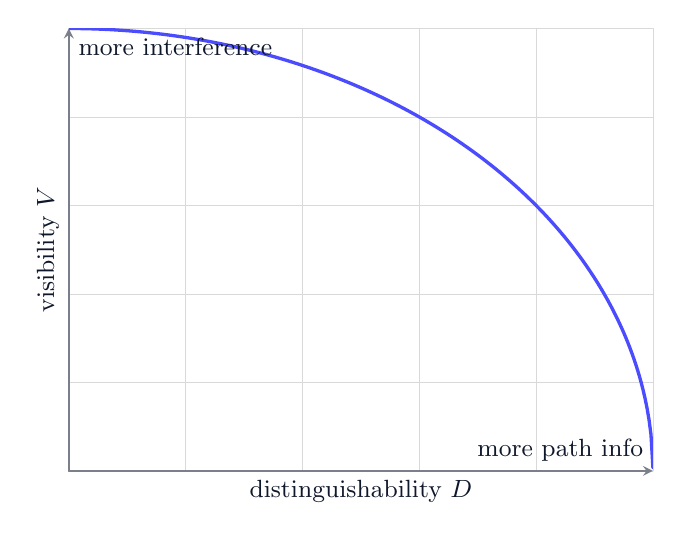
\begin{tikzpicture}
\begin{axis}[
  width=9.0cm,
  height=7.2cm,
  xlabel={distinguishability $D$},
  ylabel={visibility $V$},
  xmin=0, xmax=1,
  ymin=0, ymax=1,
  axis lines=left,
  grid=both,
  grid style={line width=.1pt, draw=gray!20},
  major grid style={line width=.2pt,draw=gray!30},
  ticks=none
]
\addplot[blue!70, very thick, domain=0:1, samples=300] {sqrt(1-x^2)};
\node[anchor=south east, font=\small] at (axis cs:1,0) {more path info};
\node[anchor=north west, font=\small] at (axis cs:0,1) {more interference};
\end{axis}
\end{tikzpicture}
\caption{Visibility--distinguishability tradeoff. In an ideal pure-state which-path model, $V^2+D^2=1$: gaining which-path information ($D$) reduces interference visibility ($V$). More realistic noise models yield $V^2+D^2\le 1$.}
\label{fig:VD}
\end{figure}

\subsection{Time-bin superposition: ``early or late'' is not classical ignorance}
Let $|E\rangle$ and $|L\rangle$ be orthonormal time-bin modes. Consider
\[
|\psi\rangle=\frac{|E\rangle+e^{\ii\theta}|L\rangle}{\sqrt{2}}.
\]
\begin{figure}[t]
\centering
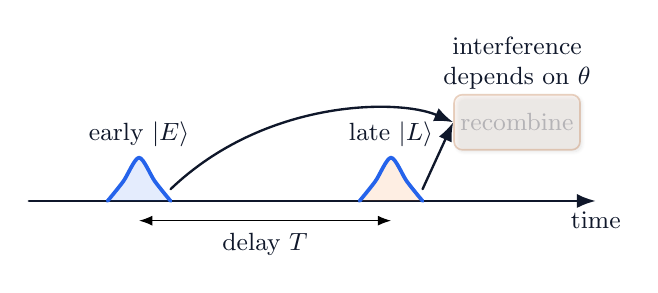
\begin{tikzpicture}[scale=1.0]
  % Time axis
  \draw[arrow] (0,0) -- (7.2,0) node[below] {time};

  % Early pulse
  \fill[accent, opacity=0.12] (1.0,0) -- plot[smooth] coordinates {(1.0,0) (1.2,0.25) (1.4,0.55) (1.6,0.25) (1.8,0)} -- cycle;
  \draw[light, smooth] plot coordinates {(1.0,0) (1.2,0.25) (1.4,0.55) (1.6,0.25) (1.8,0)};
  \node[annot] at (1.4,0.85) {early $|E\rangle$};

  % Late pulse
  \fill[accent2, opacity=0.12] (4.2,0) -- plot[smooth] coordinates {(4.2,0) (4.4,0.25) (4.6,0.55) (4.8,0.25) (5.0,0)} -- cycle;
  \draw[light, smooth] plot coordinates {(4.2,0) (4.4,0.25) (4.6,0.55) (4.8,0.25) (5.0,0)};
  \node[annot] at (4.6,0.85) {late $|L\rangle$};

  % Delay marker
  \draw[<->] (1.4,-0.25) -- (4.6,-0.25);
  \node[annot] at (3.0,-0.55) {delay $T$};

  % Recombination box
  \node[phase] (recomb) at (6.2,1.0) {recombine};
  \draw[arrow] (5.0,0.15) -- (recomb.west);
  \draw[arrow] (1.8,0.15) .. controls (3.0,1.3) and (4.7,1.3) .. (recomb.west);
  \node[annot, align=center] at (6.2,1.75) {interference\\depends on $\theta$};
\end{tikzpicture}
\caption{Time-bin encoding. A photon can be prepared in a superposition of an ``early'' wavepacket $|E\rangle$ and a ``late'' wavepacket $|L\rangle$. Measuring which bin gives 50/50, but recombining the bins reveals phase-dependent interference.}
\label{fig:time-bin}
\end{figure}

Measurement in the $\{|E\rangle,|L\rangle\}$ basis yields each with probability $1/2$, independent of $\theta$. But recombination (measuring in the $|\pm\rangle=(|E\rangle\pm|L\rangle)/\sqrt2$ basis) yields:
\[
P(+)=\left|\frac{1+e^{\ii\theta}}{2}\right|^2
=\cos^2\left(\frac{\theta}{2}\right),\qquad
P(-)=\sin^2\left(\frac{\theta}{2}\right).
\]

\subsection{Emitter--field entanglement: ``photon on/off'' can be conditional}
Consider
\[
|\Psi\rangle = \frac{|e\rangle|0\rangle + |g\rangle|1\rangle}{\sqrt{2}}.
\]
Tracing out the atom yields
\[
\rho_\text{field}
=\Tr_\text{atom}(|\Psi\rangle\langle\Psi|)
=\frac12\left(|0\rangle\langle 0| + |1\rangle\langle 1|\right).
\]
An on/off detector with efficiency $\eta$ and $p_d=0$ predicts:
\[
p_\text{on} = \Tr(\rho_\text{field}\,\Pi_\text{on}^{(\eta)})=\frac{\eta}{2}.
\]
Conditioning on measuring the atom prepares definite field states $|0\rangle$ or $|1\rangle$; thus ``photon on/off'' can be a conditional statement relative to correlated degrees of freedom.

\subsection{Mode-basis dependence: a definite photon in one mode can be a superposition in another}
Let $a_u,a_v$ be annihilation operators for orthonormal modes $u,v$ and define rotated modes:
\[
a_\pm=\frac{a_u\pm a_v}{\sqrt2}.
\]
Then $a_u^\dagger = (a_+^\dagger + a_-^\dagger)/\sqrt2$. Acting on vacuum:
\[
|1_u,0_v\rangle = a_u^\dagger|0\rangle
=\frac{1}{\sqrt2}\left(a_+^\dagger+a_-^\dagger\right)|0\rangle
=\frac{|1_+,0_-\rangle + |0_+,1_-\rangle}{\sqrt2}.
\]
So ``one photon present'' is mode-dependent; any binary on/off claim must specify the detector's mode.

\section{Where the ``contradictions'' come from (and how superposition resolves them)}
The recurring pattern is:
\begin{itemize}
  \item one measurement context asks a yes/no question about a particular basis (e.g., ``which path?'', ``which time bin?'', ``is $n=0$?''),
  \item another context asks about interference/coherence in a complementary basis.
\end{itemize}
Attempting to assign simultaneous, context-independent truth values to both sets of questions leads to apparent contradictions. Quantum theory avoids contradiction by representing the system by a state (vector or density operator) that can contain coherent superpositions, predicting outcomes via Born-rule probabilities $\Tr(\rho\,\Pi_i)$, and allowing measurement interactions (and entanglement with environments) to change which coherences are accessible.

\section{Time resolution, bandwidth, and the Planck scale (operational framing)}

\subsection{``Time window'' vs.\ ``photon present'': what a detector really does}
A real detector defines a detection \textbf{mode} (filtering + mode overlap), a detection \textbf{window} of duration $T$, and a POVM (often thresholding). Thus ``photon on in a Planck-time slice'' requires a physically realizable detector whose response has support on that timescale \emph{and} couples to the relevant ultra-broadband modes.

\subsection{``Photon in flight'': what an intermediate-time statement actually means}
The phrase ``examine the photon mid-flight'' is only meaningful once it is translated into an operational question. In standard quantum theory, between a preparation at time $t_0$ and a later measurement at time $t_1$, the system is represented by a state that evolves unitarily:
\[
\rho(t)=U(t,t_0)\,\rho(t_0)\,U^\dagger(t,t_0).
\]

\paragraph{Counterfactual vs.\ intervening measurement.}
If one does \emph{not} insert any apparatus at an intermediate time $t\in(t_0,t_1)$, then statements like ``the photon was \emph{really} on/off at time $t$'' are counterfactual: they refer to an outcome of a measurement that was not performed. What is well-defined are probabilities for \emph{hypothetical} measurements one \emph{could} perform at time $t$.

\paragraph{Intermediate measurement as a POVM (and its backaction).}
To ``look'' mid-flight, one must couple the field to a device during some time window and thereby implement a POVM $\{E_k\}$ at time $t$. The Born rule gives
\[
p(k;t)=\Tr\!\big(\rho(t)\,E_k\big).
\]
If the measurement is actually performed, the post-measurement state conditioned on outcome $k$ is updated by Kraus operators $\{M_k\}$ (with $E_k=M_k^\dagger M_k$):
\[
\rho(t)\ \longrightarrow\ \rho_k(t)=\frac{M_k\,\rho(t)\,M_k^\dagger}{p(k;t)}.
\]
This \emph{changes} the statistics of later measurements at $t_1$. In interferometers, for example, even weak which-path probes reduce coherence and thus reduce visibility (quantitatively captured by overlap factors like $\gamma$ and inequalities like $V^2+D^2\le 1$).

\paragraph{An explicit ``mid-flight probe'' model: unsharp which-path measurement.}
It is useful to see the disturbance quantitatively in the simplest nontrivial setting: a single-photon in a two-path superposition. Let $\{|A\rangle,|B\rangle\}$ denote orthonormal path states (arms of a Mach--Zehnder). Consider the pre-measurement state at time $t$:
\[
\rho(t)=
\begin{pmatrix}
\rho_{AA} & \rho_{AB}\\
\rho_{BA} & \rho_{BB}
\end{pmatrix}
\quad \text{in the basis } \{|A\rangle,|B\rangle\}.
\]
Now insert a weak which-path monitor in arm $B$ whose \emph{outcomes} are:
``no record'' ($k=0$) and ``path-B record'' ($k=1$). One simple instrument realizing this is:
\[
M_0 = |A\rangle\langle A| + \sqrt{1-\lambda}\,|B\rangle\langle B|,
\qquad
M_1 = \sqrt{\lambda}\,|B\rangle\langle B|,
\]
with measurement strength $\lambda\in[0,1]$.
The POVM elements are
\[
E_0=M_0^\dagger M_0 = |A\rangle\langle A| + (1-\lambda)|B\rangle\langle B|,
\qquad
E_1=M_1^\dagger M_1 = \lambda |B\rangle\langle B|.
\]
If one \emph{ignores} the intermediate outcome (i.e.\ does not condition on $k$), the state evolves under the completely positive trace-preserving map
\[
\rho \longrightarrow \rho' = \sum_{k=0,1} M_k \rho M_k^\dagger.
\]
A short calculation shows that the populations are unchanged, but the coherence is reduced:
\[
\rho'_{AA}=\rho_{AA},\quad \rho'_{BB}=\rho_{BB},\quad
\rho'_{AB}=\sqrt{1-\lambda}\,\rho_{AB},\quad
\rho'_{BA}=\sqrt{1-\lambda}\,\rho_{BA}.
\]
Thus any later interference fringes that depend on $\rho_{AB}$ are suppressed by the factor $\sqrt{1-\lambda}$. In other words, ``looking a little'' mid-flight means \emph{destroying a little} of the phase coherence that produces interference.

\paragraph{Planck time does not grant noninvasive snapshots.}
The role of the Planck time in this discussion is not that it provides a privileged intermediate instant at which the photon becomes ``more real'' or ``more inspectable.'' Rather, to implement a measurement in an ultra-short window $\Delta t$ one needs an apparatus with correspondingly large bandwidth and strong coupling; for $\Delta t$ pushed toward $t_P$, heuristic arguments suggest energies approaching the Planck scale and unavoidable gravitational backreaction. In that regime, the standard quantum-optics instrument models above (and even the fixed-background notion of ``a photon traveling in spacetime'') may cease to apply, but this does not amount to a free pass to assign definite mid-flight properties without backaction.

\paragraph{So is the photon ``only mathematically represented'' in flight?}
Between measurements, the state $\rho(t)$ is indeed a mathematical object---but it is not ``mere'' math: it encodes experimentally testable predictions for any measurement you choose to implement at time $t$ or later. What fails is the classical move of treating $\rho(t)$ as a hidden record of a definite trajectory or a definite on/off property independent of measurement context.

\subsection{Fourier-limited pulses: explicit bandwidth--duration relation}
For a transform-limited pulse with temporal envelope $g(t)$ and spectrum $\tilde g(\omega)$, rms widths satisfy
\[
\Delta t\,\Delta\omega \ge \frac12,
\]
with equality for Gaussians. If $\Delta t = t_P$, then $\Delta\omega \gtrsim 1/(2t_P)\sim 10^{43}\,\mathrm{s^{-1}}$, corresponding to energies per quantum of order $\hbar\Delta\omega \sim \hbar/t_P = E_P$.

\begin{figure}[t]
\centering
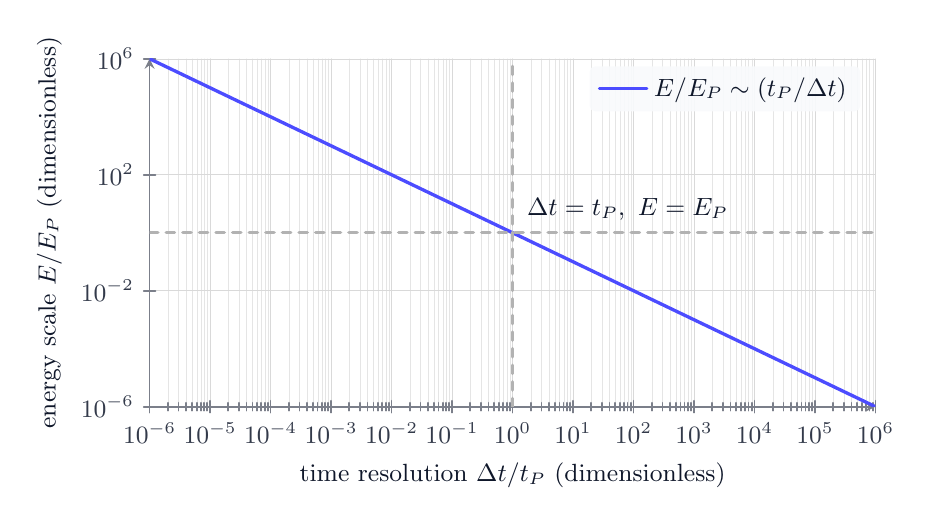
\begin{tikzpicture}
\begin{loglogaxis}[
  width=10.8cm,
  height=6.0cm,
  xlabel={time resolution $\Delta t/t_P$ (dimensionless)},
  ylabel={energy scale $E/E_P$ (dimensionless)},
  xmin=1e-6, xmax=1e6,
  ymin=1e-6, ymax=1e6,
  axis lines=left,
  grid=both,
  grid style={line width=.1pt, draw=gray!20},
  major grid style={line width=.2pt,draw=gray!30},
  legend style={at={(0.98,0.98)}, anchor=north east, font=\small}
]
\addplot[blue!70, very thick, domain=1e-6:1e6, samples=200] {1/x};
\addlegendentry{$E/E_P \sim (t_P/\Delta t)$}
\addplot[gray!60, dashed] coordinates {(1e-6,1) (1e6,1)};
\addplot[gray!60, dashed] coordinates {(1,1e-6) (1,1e6)};
\node[font=\small, anchor=south west] at (axis cs:1.2,1.2) {$\Delta t=t_P,\ E=E_P$};
\end{loglogaxis}
\end{tikzpicture}
\caption{Heuristic scaling behind Planck-time caution. In dimensionless units, resolving shorter times ($\Delta t/t_P \ll 1$) pushes characteristic energy scales upward roughly as $E/E_P \sim t_P/\Delta t$. This motivates why extrapolating familiar photon+detector models deep below $t_P$ is expected to encounter gravitational backreaction.}
\label{fig:planck-scaling}
\end{figure}

\subsection{Why this does not imply ``photons flip on/off each \texorpdfstring{$t_P$}{tP}''}
The reasoning says that probing such short times pushes one to Planckian energies and gravitational backreaction, so naive quantum-optics models likely fail. It does \emph{not} say that physical fields evolve in discrete ticks, that a photon has an intrinsic binary on/off variable that updates at $t_P$, or that standard quantum superposition ceases to apply.

\section{FAQ (general public)}

\paragraph{Q: Is a photon a tiny ball flying through space?}
\textbf{A:} Not in the way a baseball is. In quantum optics, a photon is an excitation of a \emph{field mode}. Many experiments produce particle-like \emph{clicks}, and those clicks are discrete. But between source and detector, the best description is a quantum state that predicts probabilities for clicks in different detectors, not a little ball with a definite path.

\paragraph{Q: When the detector does not click, does that mean the photon was ``off''?}
\textbf{A:} No-click means ``no registered event in this time window.'' That can happen because the field was vacuum in the relevant mode, \emph{or} because of inefficiency/loss, timing mismatch, or mode mismatch. This is why we model detection as a POVM and include efficiency and dark counts.

\paragraph{Q: When the detector clicks, does that mean there was exactly one photon?}
\textbf{A:} Not necessarily. Many detectors are threshold (on/off) devices: one photon and two photons both produce the same ``on'' outcome. Also, dark counts can produce clicks even when the field state is vacuum.

\paragraph{Q: What does ``superposition'' mean in plain language?}
\textbf{A:} It is a special kind of ``both'' that can create \emph{interference patterns} when alternatives are recombined. It is not just ``we don't know which.'' A random mixture does not produce the same interference effects. Section~3 gives both an intuitive definition and the precise density-matrix/coherence definition.

\paragraph{Q: Does a photon have a definite position while it is traveling (``in flight'')?}
\textbf{A:} The theory gives a definite rule for what happens \emph{if you measure} at some intermediate time, and it gives definite probabilities for later measurements. But attributing a single measurement-independent ``where it really is'' to the photon between measurements is not operationally well-defined unless you specify the measurement you mean. If you actually try to measure mid-flight, the measurement interaction can change later interference statistics (backaction).

\paragraph{Q: Does ``observation'' mean a human mind changes reality?}
\textbf{A:} In physics, ``observation'' means a physical interaction that leaves a record (in a detector, environment, memory register, etc.). The relevant effect is coupling/entanglement, not human consciousness.

\paragraph{Q: Why can adding a third polarizer increase the amount of light?}
\textbf{A:} Because quantum states (and also classical polarization vectors) transform by projections that depend on orientation. Two crossed polarizers block light, but an intermediate polarizer rotates the polarization step-by-step so that some amplitude survives. The single-photon calculation reproduces the same result.

\paragraph{Q: What does Planck time mean for these questions?}
\textbf{A:} Planck time is a natural quantum-gravity scale. It does not by itself imply discrete time ticks or that photons ``update'' every $t_P$. The cautious message is: trying to operationally probe times far below $t_P$ likely requires Planckian energies, where gravitational backreaction cannot be ignored and the usual photon+detector models may break down.

\paragraph{Q: So is the photon ``only mathematical'' between source and detector?}
\textbf{A:} The quantum state is a mathematical object, but it is not arbitrary: it is a compact representation of experimentally testable predictions. Calling it ``only math'' becomes misleading if it suggests there is \emph{no} physical content. The physical content is precisely the pattern of probabilities it predicts for all possible measurements you could implement.

\section{Critical physicist remarks (caveats and common pitfalls)}

This section collects the kinds of objections, clarifications, and ``what exactly do you mean?'' questions that a skeptical physicist will ask. The intent is not to weaken the operational claims above, but to keep them precise: the core results are about \emph{measurement-defined} questions (POVMs) applied to \emph{mode-defined} degrees of freedom.

\subsection{Planck time: dimensional scale vs.\ operational cutoff}
\begin{itemize}
  \item \textbf{Dimensional analysis is not a theorem.} The combination $t_P=\sqrt{\hbar G/c^5}$ is the unique time scale built from $(\hbar,G,c)$, but that alone does not prove a minimum time step or a discrete clock in nature.
  \item \textbf{The black-hole argument is heuristic.} The estimate $\Delta t \gtrsim t_P$ comes from combining Fourier bandwidth ideas with a classical Schwarzschild radius and a crude localization scale. It is a plausibility bound about when gravitational backreaction cannot be ignored, not an experimentally established limit. Related arguments appear in classic measurement-limit discussions \cite{salecker_wigner,mead}.
  \item \textbf{Be explicit about what is being localized.} ``Resolving a time interval'' can mean (i) resolving the arrival time of a click, (ii) estimating a phase in a frequency standard, (iii) constraining a time parameter in a Hamiltonian, etc. These are different operational tasks with different resource scalings (estimation theory matters).
\end{itemize}

\subsection{Time--energy ``uncertainty'': avoid overclaiming}
\begin{itemize}
  \item \textbf{Time is not an operator in standard nonrelativistic QM.} The familiar Robertson relation $\Delta A\,\Delta B \ge \tfrac12|\langle[A,B]\rangle|$ applies to pairs of operators. ``Energy--time uncertainty'' is subtler and is best framed in terms of (i) Fourier bandwidth of wavepackets, (ii) dynamical timescales set by Hamiltonians, or (iii) bounds from parameter estimation. Conflating these with a commutator relation is a common source of sloppy claims.
  \item \textbf{Bandwidth is the clean statement here.} In this paper, the $\Delta t\,\Delta\omega \gtrsim 1$ statement is a Fourier-limited wavepacket relation (or a statement about signal processing), not a fundamental operator uncertainty principle.
\end{itemize}

\subsection{Photons are mode excitations; localization is subtle}
\begin{itemize}
  \item \textbf{A photon is not an object with a position operator like a massive particle.} In relativistic quantum theory, the notion of a ``particle'' is tied to a mode decomposition; sharply localized photon states and a universally agreed photon position observable are subtle topics. Operationally, experiments access mode overlaps and field correlation functions.
  \item \textbf{Mode definitions are part of the measurement.} Our $a_f=\int d\omega\,f(\omega)a(\omega)$ construction makes this explicit: the question ``is there a photon?'' is always ``is there a photon in \emph{this} mode that my apparatus couples to?'' Changing filters, apertures, local-oscillator shapes, cavity boundary conditions, or timing gates changes the effective mode and thus changes what ``on/off'' means.
\end{itemize}

\subsection{Detector models: POVMs are effective, device-dependent descriptions}
\begin{itemize}
  \item \textbf{On/off POVMs are idealizations.} Real detectors have timing jitter, dead time, afterpulsing, saturation, wavelength dependence, and finite bandwidth. All of these modify the effective POVM. The $(1-\eta)^n$ ``no-click'' model is a useful baseline, not a universal truth.
  \item \textbf{A ``click'' is not the same as ``one photon.''} A threshold detector cannot number-resolve; multi-photon states can produce the same ``on'' outcome as single-photon states. Conversely, a single-photon state can fail to click due to losses. Interpreting click/no-click as a literal microscopic particle counter is a common category error in discussions that aim to be foundational.
  \item \textbf{Vacuum is not ``nothing.''} Field vacuum has fluctuations and nontrivial correlations; what matters operationally is whether your detector responds above its noise floor in a specified window. ``Dark counts'' are a classical manifestation of this: even in the absence of signal photons, detectors can click.
\end{itemize}

\subsection{Interference vs.\ which-path: complementarity is quantitative, and definitions matter}
\begin{itemize}
  \item \textbf{Equality requires idealizations.} The clean relation $V^2+D^2=1$ holds in the pure-state model with equal arm weights and the specific distinguishability definition used here. More realistic situations (mixed environments, unequal splitting, additional noise) yield $V^2+D^2\le 1$; a standard reference is Englert's inequality \cite{englert}.
  \item \textbf{Which-path information is about accessibility.} It is possible for path information to be \emph{in principle} present in some environment degree of freedom but not practically retrievable, or to be ``erased'' by conditioning on another measurement. This is not paradoxical; it is conditional probability in a larger Hilbert space.
  \item \textbf{Be wary of counterfactual claims.} Statements like ``the photon really went through arm A'' are not operationally meaningful unless tied to a specific measurement that would establish that fact without destroying the interference being discussed.
\end{itemize}

\subsection{Complementarity, contextuality, and nonlocality are different claims}
\begin{itemize}
  \item \textbf{Complementarity:} incompatible measurement contexts (e.g.\ which-path vs.\ interference) cannot be simultaneously realized with full sharpness in one experimental configuration.
  \item \textbf{Contextuality:} the outcome assignment for an observable cannot be made independent of the set of compatible observables measured alongside it (Kochen--Specker-type constraints) \cite{kochen_specker}. Not every ``wave/particle'' discussion is a contextuality proof.
  \item \textbf{Nonlocality:} Bell-type correlations that cannot be explained by local hidden-variable models. This paper does not attempt a Bell test; it sticks to single-system operational predictions.
\end{itemize}

\subsection{Analogy limits: projection in real space vs.\ projection in Hilbert space}
\begin{itemize}
  \item \textbf{The ``square circle'' story is an analogy, not a hidden-variable model.} The cylinder example is meant to train the intuition that incompatible ``views'' can come from information-discarding maps. In quantum mechanics, the relevant ``space'' is Hilbert space, and measurement is a physical interaction, not merely a change in viewpoint.
  \item \textbf{Not all measurements are projective.} Realistic measurement descriptions are POVMs; projectors are a special ideal case. The operational conclusions here are therefore stated in POVM language wherever possible.
\end{itemize}

\section{Conclusion}
\begin{enumerate}
  \item ``Photon on/off'' is shorthand for a mode-defined and measurement-defined predicate.
  \item With explicit detector POVMs, on/off outcomes are straightforward to compute and show no inconsistency.
  \item Apparent contradictions most often come from importing classical assumptions of measurement-independent, simultaneously definite properties for incompatible observables.
  \item Planck time is a natural quantum-gravity scale; heuristic arguments suggest operational probes below $t_P$ require Planckian energies, but this does not by itself imply time discreteness or binary ``flip'' dynamics.
\end{enumerate}

\appendix

\section{On/off POVM derivation for inefficiency}
If each photon is independently detected with probability $\eta$, then with $n$ photons the probability of \emph{no} detection is $(1-\eta)^n$. For a number-diagonal state $\rho=\sum_n p_n |n\rangle\langle n|$,
\[
p_\text{off}=\sum_{n=0}^\infty p_n(1-\eta)^n
=\Tr\!\left(\rho\sum_{n=0}^\infty (1-\eta)^n |n\rangle\langle n|\right).
\]
Thus the operator in parentheses is the POVM element $\Pi_\text{off}^{(\eta)}$.

\section{Two-mode basis rotation identity}
For orthonormal modes $u,v$, define $a_\pm=(a_u\pm a_v)/\sqrt2$. Then
\[
a_u^\dagger = \frac{a_+^\dagger+a_-^\dagger}{\sqrt2}
\Rightarrow
a_u^\dagger|0\rangle = \frac{|1_+,0_-\rangle + |0_+,1_-\rangle}{\sqrt2}.
\]

\begin{thebibliography}{9}

\bibitem{gerry_knight}
C.~Gerry and P.~Knight,
\emph{Introductory Quantum Optics}.

\bibitem{walls_milburn}
D.~F.~Walls and G.~J.~Milburn,
\emph{Quantum Optics}.

\bibitem{mandel_wolf}
L.~Mandel and E.~Wolf,
\emph{Optical Coherence and Quantum Optics}.

\bibitem{nielsen_chuang}
M.~A.~Nielsen and I.~L.~Chuang,
\emph{Quantum Computation and Quantum Information}.

\bibitem{peres}
A.~Peres,
\emph{Quantum Theory: Concepts and Methods}.

\bibitem{helstrom}
C.~W.~Helstrom,
\emph{Quantum Detection and Estimation Theory}
(Academic Press, 1976).

\bibitem{englert}
B.-G.~Englert,
``Fringe Visibility and Which-Way Information: An Inequality,''
\emph{Phys.\ Rev.\ Lett.} \textbf{77}, 2154 (1996).

\bibitem{salecker_wigner}
H.~Salecker and E.~P.~Wigner,
``Quantum limitations of the measurement of space-time distances,''
\emph{Phys.\ Rev.} \textbf{109}, 571 (1958).

\bibitem{mead}
C.~A.~Mead,
``Possible connection between gravitation and fundamental length,''
\emph{Phys.\ Rev.} \textbf{135}, B849 (1964).

\bibitem{kochen_specker}
S.~Kochen and E.~P.~Specker,
``The problem of hidden variables in quantum mechanics,''
\emph{J.\ Math.\ Mech.} \textbf{17}, 59 (1967).

\end{thebibliography}

\end{document}


